\documentclass[compress]{beamer}
%for printing or having a crappy pdf reader backup
%\documentclass[handout]{beamer}
\mode<presentation>
\usetheme{Madrid}


\usecolortheme[RGB={128,128,128}]{structure}
\definecolor{my_gray}{RGB}{105,105,105}
\setbeamercolor{khumna}{fg=white,bg=my_gray}
%teal \usecolortheme[RGB={0,128,128}]{structure}
%\useoutertheme{miniframes}
\useinnertheme{default}
\usepackage{color}
\definecolor{Maroon}{RGB}{80,0,0}
\definecolor{BurntOrange}{RGB}{204,85,0}
\usepackage{setspace}
\usepackage{amsmath}
\usepackage{amsthm}
\usepackage{amsfonts}
\usepackage{amssymb}
\usepackage{verbatim}
\usepackage{array}
\usepackage{graphicx}
\usepackage{subfigure}
\usepackage{colortbl}
%\usepackage[retainorgcmds]{IEEEtrantools}
\usepackage{wrapfig}
\usepackage[figurename=,tablename=]{caption}
\usepackage{multirow}
\setbeamercolor{normal text}{fg=black}
\setbeamercovered{dynamic}
\beamertemplatetransparentcovereddynamicmedium
%\usepackage{chronology}
\setbeamertemplate{caption}[numbered]
\usepackage{colortbl}
\newcommand {\mathsym}[1]{{}}
\newcommand {\unicode}{{}}
\newcommand{\om}{\boldsymbol{\Omega}}
\newcommand{\etal}{{\it et al.\,}}
\newcommand{\vr}{\vec{r}}
\newcommand{\vo}{\vec{\Omega}}
\newcolumntype{L}{>{\centering\arraybackslash}m{3cm}}
\newcommand{\tcr}[1]{\textcolor{red}{#1}}
%Creating a norm command
\newcommand{\norm}[1]{\left\lVert#1\right\rVert}
%Allow page breaks within align
\allowdisplaybreaks
%Putting logo and banner in title and adding banner
\usepackage[absolute]{textpos}
%Code
\usepackage{listings}
\usepackage{epstopdf}
\usepackage{pdfpages}
\newlength \figwidth
\setlength \figwidth {0.5\textwidth}

\newcommand{\backupbegin}{
   \newcounter{finalframe}
   \setcounter{finalframe}{\value{framenumber}}
}
\newcommand{\backupend}{
   \setcounter{framenumber}{\value{finalframe}}
}

\addtobeamertemplate{frametitle}{}
{
	\begin{textblock*}{100mm}(0.85\textwidth,-1cm)
	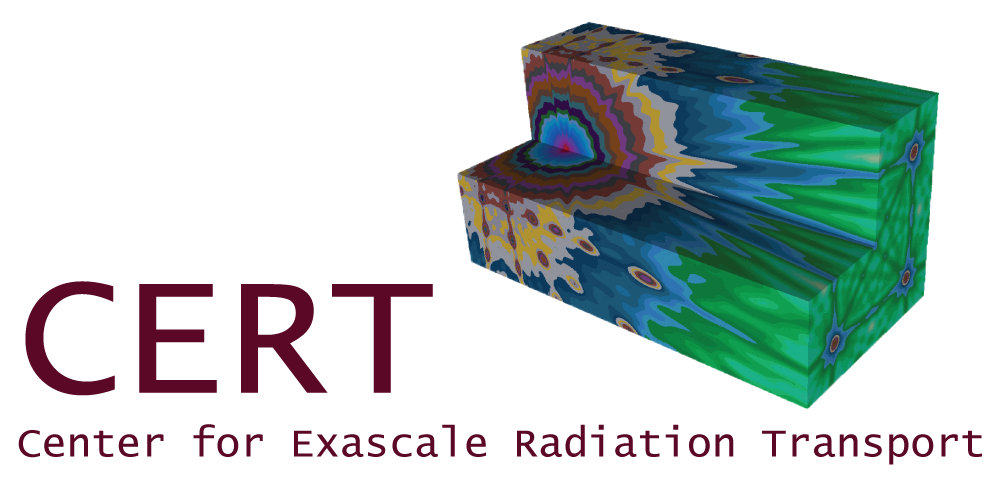
\includegraphics[height = 1cm,width=2cm]{figures/cert_logo_maroon.png}
	\end{textblock*}
}
\beamertemplatenavigationsymbolsempty



\begin{document}
%	

\title[Load Balancing]{Load Balancing Unstructured Meshes for Massively Parallel Transport Sweeps}
\author[Ghaddar]{Tarek Ghaddar \\  Dr. Jean Ragusa}
\institute[TAMU]{Texas A\&M University}
%\committee{Morel,Popov}{Dr. Jim Morel \\ Dr. Bojan Popov}
\date[April 5, 2016]

{
\setbeamertemplate{headline}{}
\begin{frame}
\vspace{-1.1cm}
	\begin{figure}[t]
		\centering
			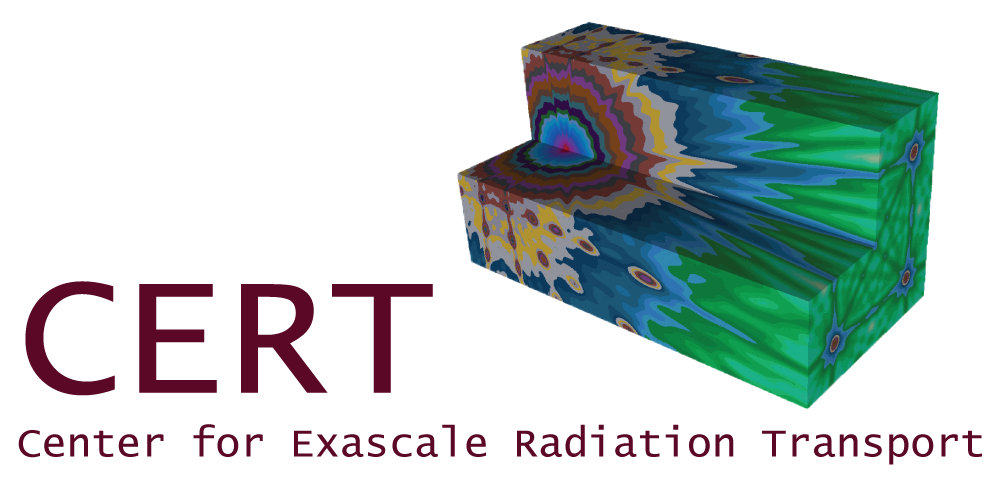
\includegraphics[width=.25\textwidth]{figures/cert_logo_maroon.png}
	\end{figure}
\vspace{-0.75cm}
\titlepage
\end{frame}
}

\setbeamertemplate{footline}
{

%\vspace{-0.1ex}
\begin{beamercolorbox}[wd=\textwidth,ht=3.5ex]{khumna}

\includegraphics[width = 0.95\textwidth]{figures/cert_banner.pdf}
	%\begin{textblock*}{10mm}(0.95\textwidth,10cm)
	\insertframenumber/\inserttotalframenumber
	%\end{textblock*}
\end{beamercolorbox}
%\begin{beamercolorbox}[wd=0.05\textwidth,ht=3.5ex]{khumna}

%\end{beamercolorbox}
}

\begin{frame}[t]\frametitle{Project Components and Integration}
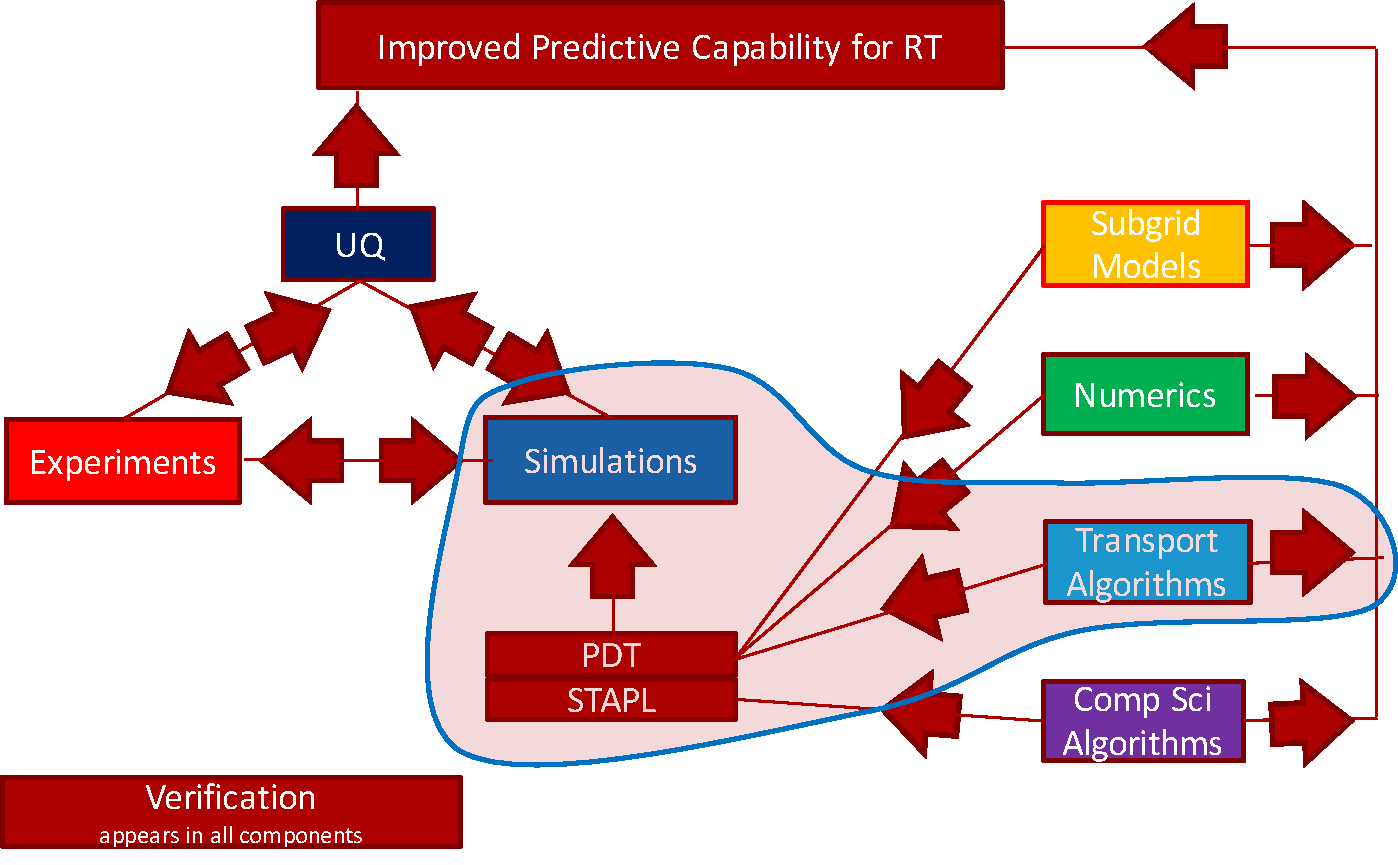
\includegraphics[scale = 0.45 ]{figures/Integration_Slide.pdf}
\end{frame}


\begin{frame}
\tableofcontents
\end{frame}

\section{Introduction}
%\subsection{}
\begin{frame}[t]\frametitle{Motivation}
	\begin{block}{}
	\begin{itemize}
		\item When running any massively parallel code, load balancing is a priority in order to achieve the best possible parallel efficiency.
		\item  A load balanced problem has an equal number of degrees of freedom per processor.
		\item Load balancing a logically Cartesian mesh is ``not difficult", as the user specifies the number of cells being used.
		\item In an unstructured mesh, the user cannot always specify the number of cells they want per processor, and obtaining a load balanced problem is more difficult.
		\item The goal is to implement a load balancing algorithm for unstructured meshes in PDT.
	\end{itemize}
	\end{block}
\end{frame}

\begin{frame}[t]\frametitle{The Triangle Mesh Generator}
	\begin{block}{}
	\begin{itemize}
		\item Unstructured meshes in PDT are generated in 2D using the Triangle Mesh Generator.
		\item These can be extruded to create 3D meshes.
	\end{itemize}	
	\end{block}
	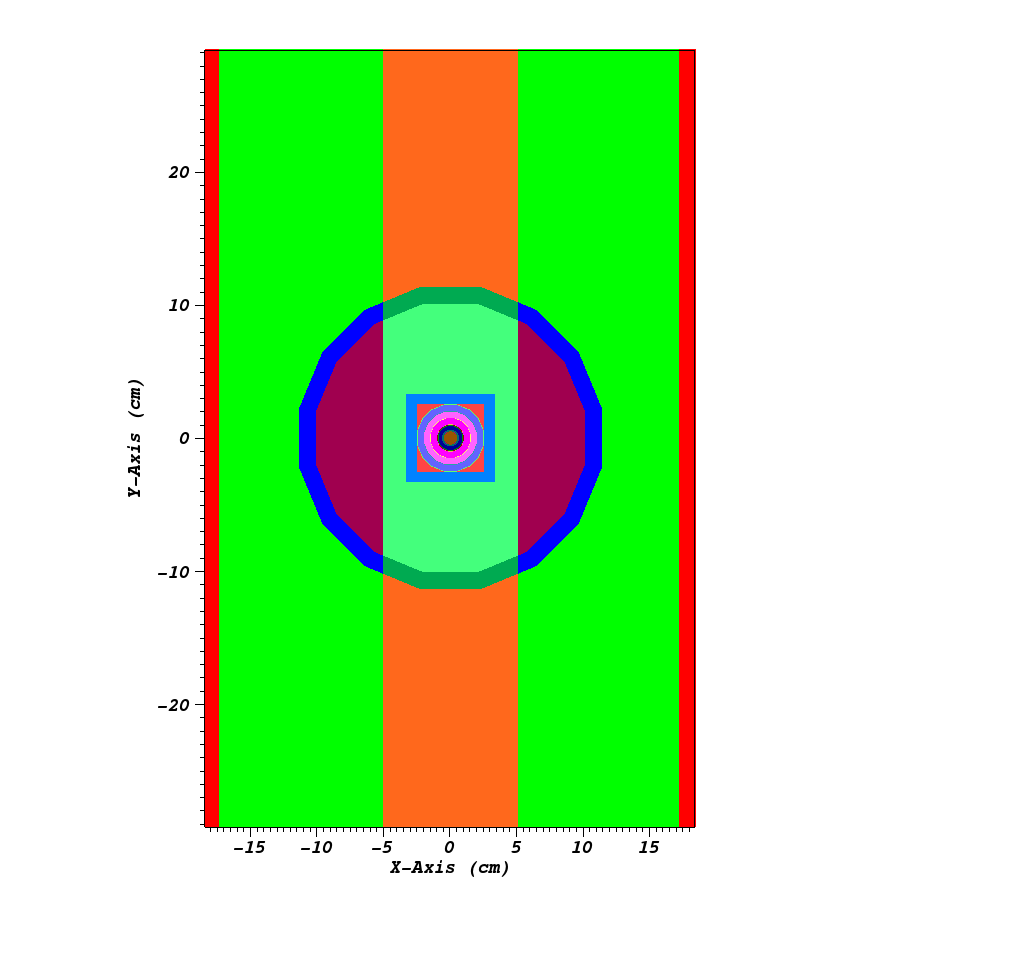
\includegraphics[scale = 0.15]{figures/IM12DPoly.png}
	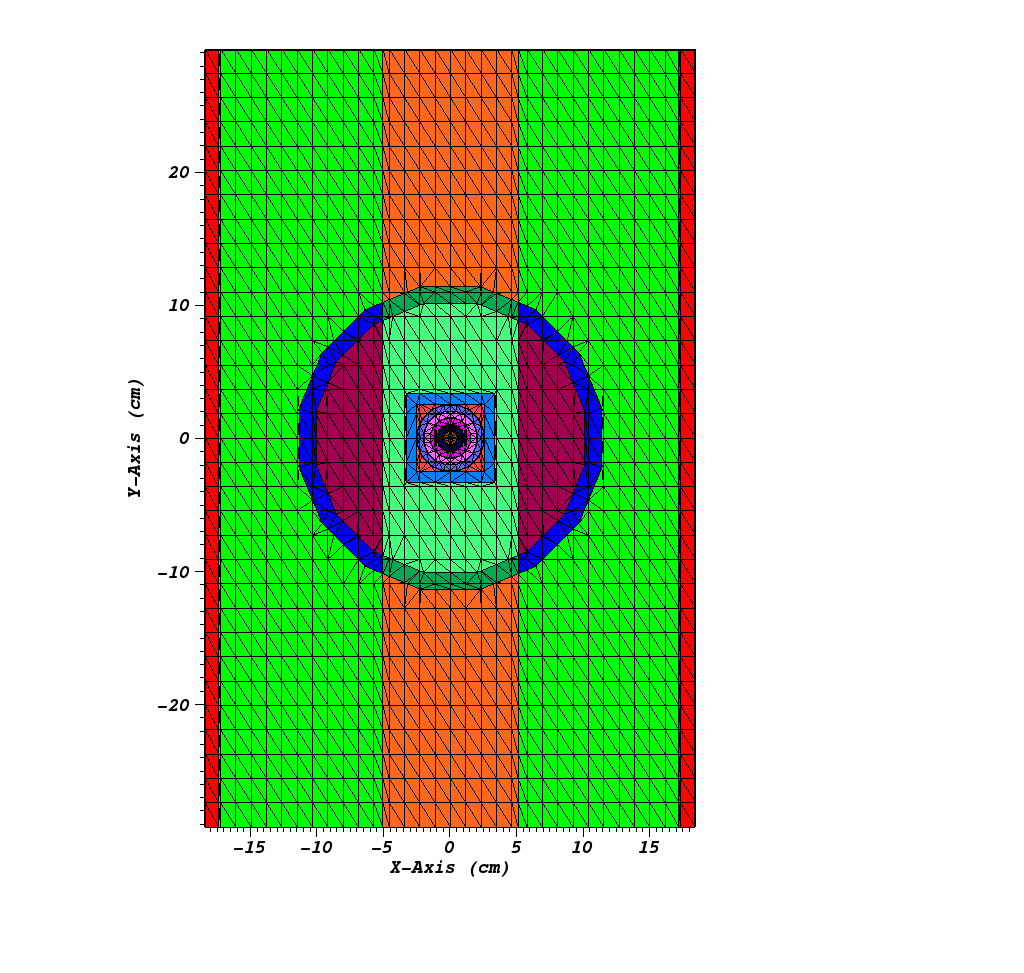
\includegraphics[scale = 0.15]{figures/IM12DMesh.png}
\end{frame}

\section{Load Balance Algorithm}
%\subsection{}

\begin{frame}[t]\frametitle{Partitioning for an Unstructured Mesh}
\begin{block}{}
	\begin{itemize}
	\item The user inputs coordinates for cut lines in the X and Y directions.
	\item The cut lines will determine the number of ``subsets" the problem is partitioned into.
	\item Optimizing the location of these cut lines is the basis of the load balancing algorithm.
	\item A ``subset" is an orthogonal unit that is formed by intersecting cut lines.
	\end{itemize}
\end{block}
\end{frame}

\begin{frame}[t]\frametitle{The Subset}
\centering
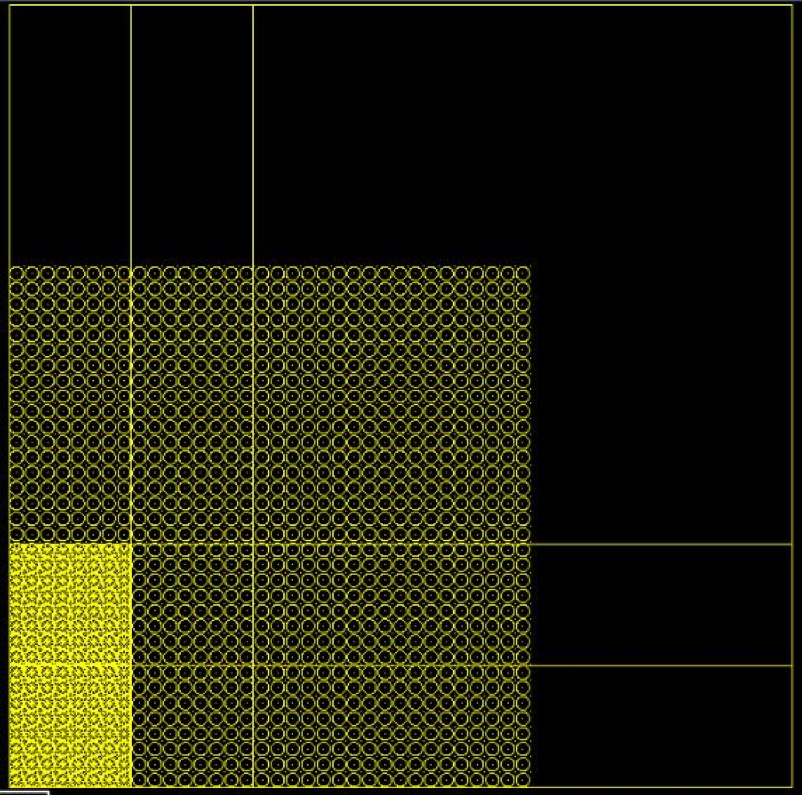
\includegraphics[width = 12 cm, height = 7 cm ]{figures/subsetlattice.png}
\end{frame}

\begin{frame}[t]\frametitle{ Goal and Definitions}
	\begin{block}{}
	
		\begin{itemize}
			\item \textbf{Goal:} Obtain an equal number of cells per processor, which for our purposes means an equal number of cells per subset.
			\item Achieved by optimizing the location of $X_i$ and $Y_j$, the location of the cut lines.
			%\item We define the load balance metric, $f$.
			\item \textbf{Define}:
			\begin{itemize}
			\item $N_{ij}$: The number of cells  in subset ${i,j}$
			%\item Cut Lines: $X_i, Y_j$, $1 <= i <= I-1$, $1 <= j <= J-1$
			\item $f =\frac{\underset{ij}{\text{max}}(N_{ij})}{\frac{N_{tot}}{I\cdot J}}$
			\item $f_I = \underset{i}{\text{max}}[\sum_{j} N_{ij}]/\frac{N_{tot}}{I}$
			\item $f_J = \underset{j}{\text{max}}[\sum_{i} N_{ij}]/\frac{N_{tot}}{J}$
			\end{itemize}
		\end{itemize}
	\end{block}
\end{frame}

\begin{frame}[t]\frametitle{Load Balancing Algorithm}
\vspace{-0.5 cm}
\begin{block}{}
\lstinputlisting[language = C++, basicstyle = \footnotesize]{loadbalance.cc}
\end{block}
\end{frame}

\begin{frame}[t]\frametitle{Redistribution Function}
\centering
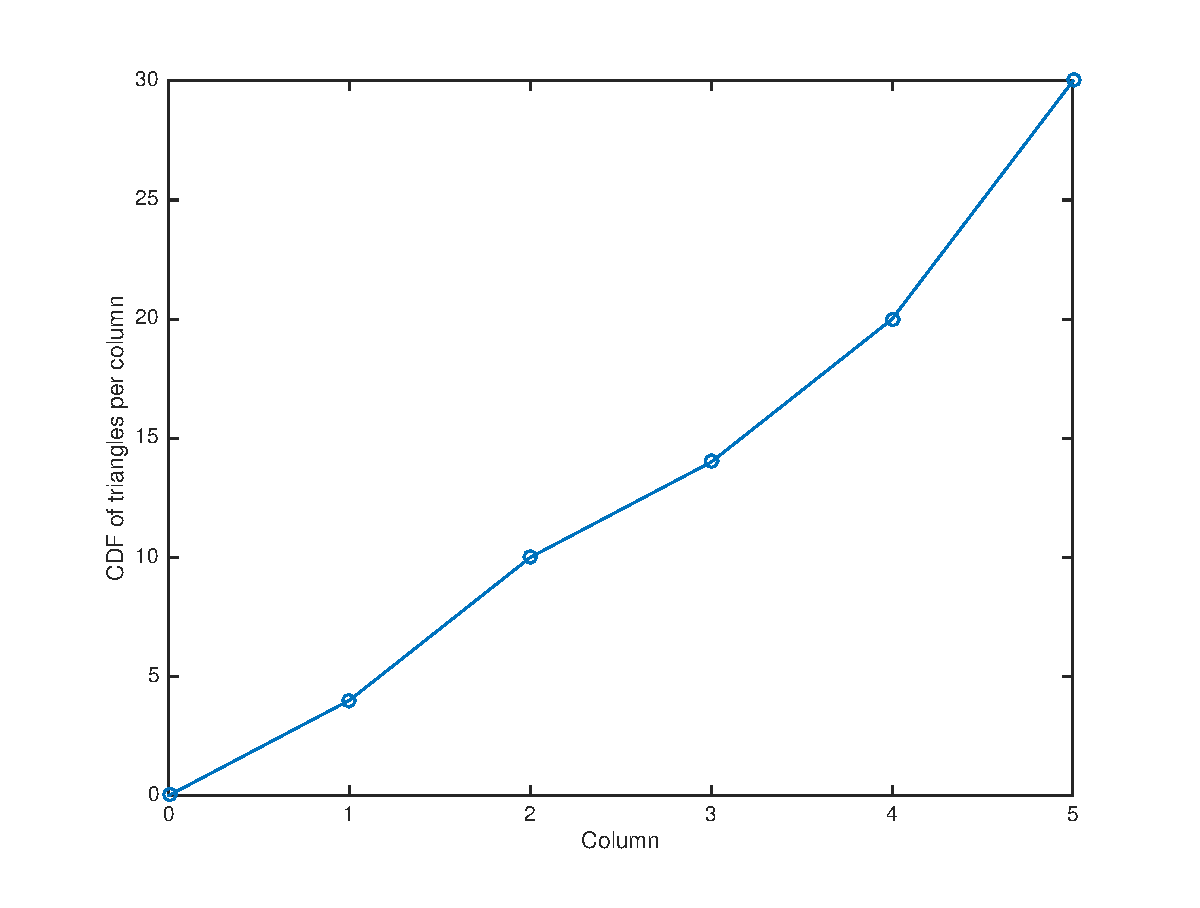
\includegraphics[scale = 0.5]{figures/before_redistribute.eps}
\end{frame}

\begin{frame}[t]\frametitle{Redistribution Function}
\centering
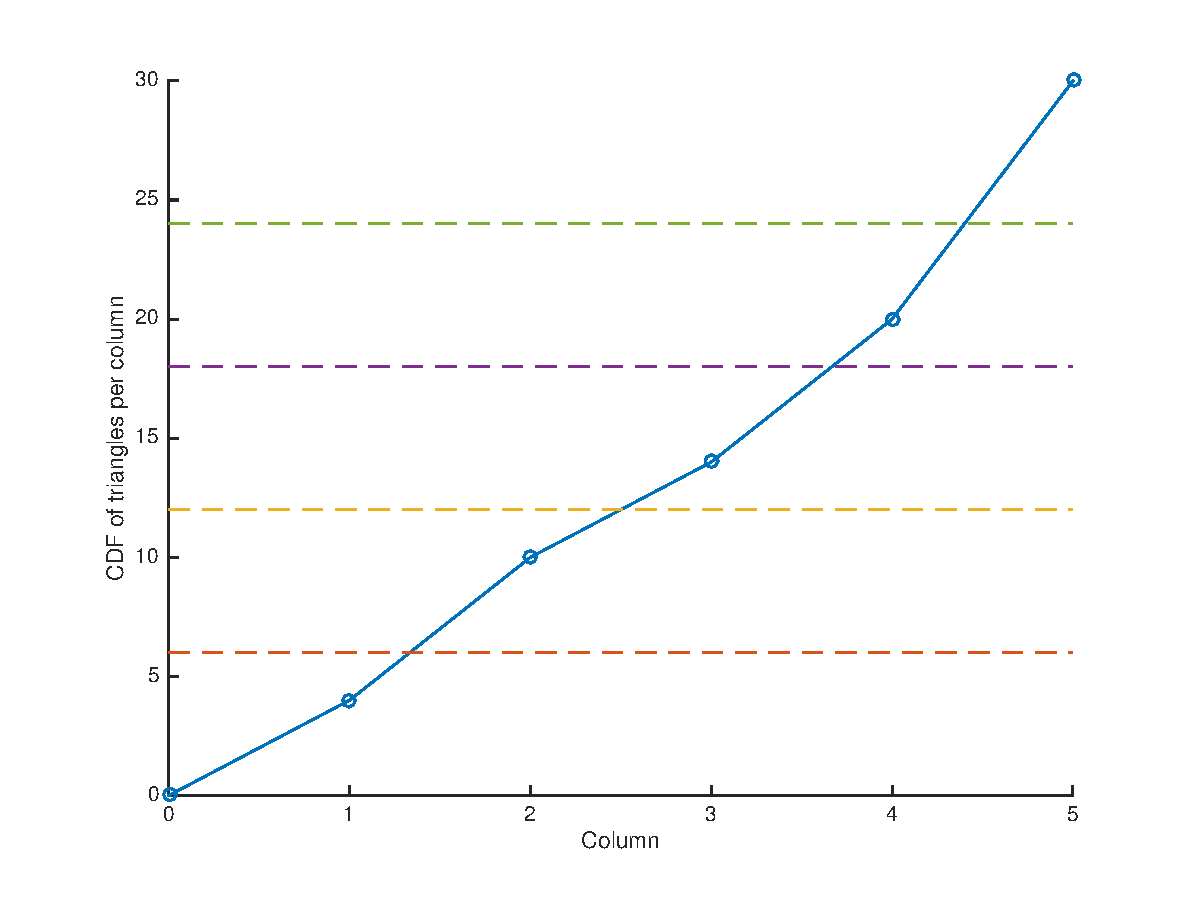
\includegraphics[scale = 0.5]{figures/after_redistribute.eps}
\end{frame}

\begin{frame}[t]\frametitle{Example}
\begin{minipage}{0.15\textwidth}
\begin{footnotesize}
Iter 0 \\
$f$ = 7.20583 
\end{footnotesize}
\end{minipage}
\begin{minipage}{0.8\textwidth}
\centering
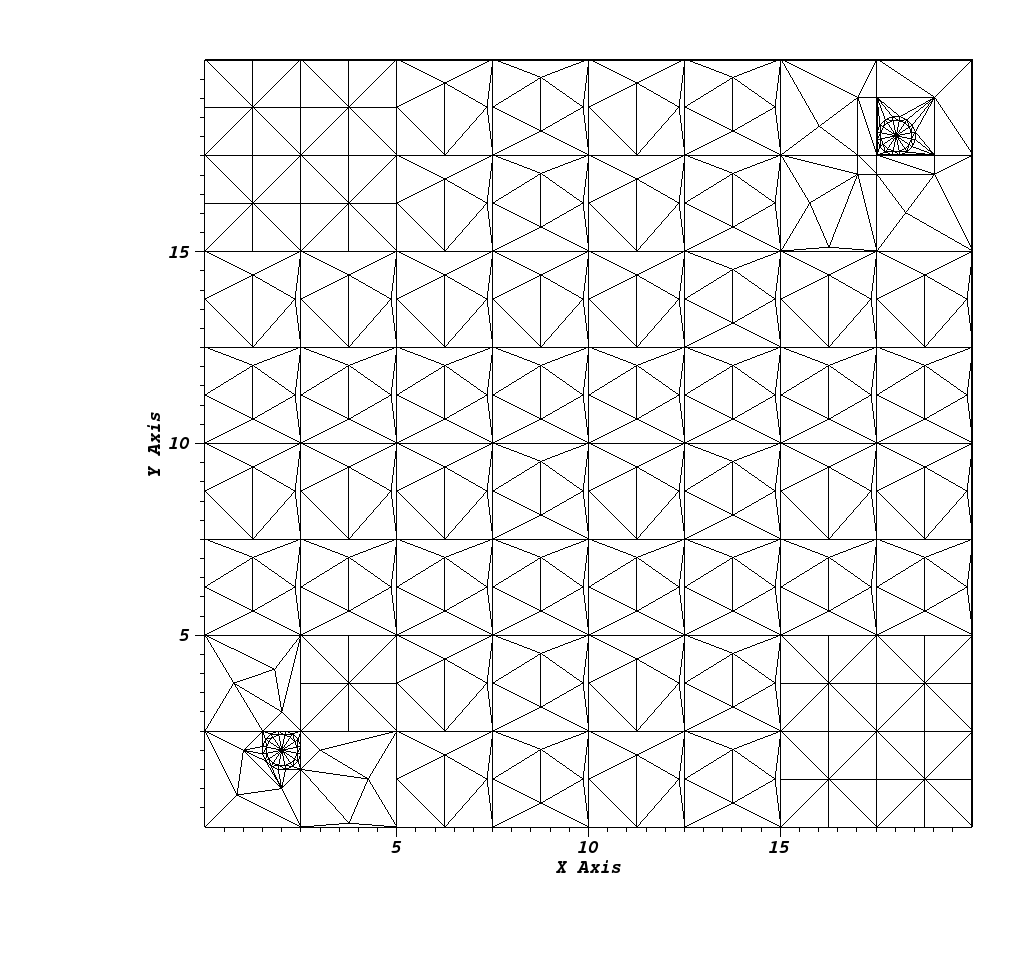
\includegraphics[scale = 0.22]{figures/redistribute_before.png}
\end{minipage}
\end{frame}

\begin{frame}[t]\frametitle{Example}
\begin{minipage}{0.15\textwidth}
\begin{footnotesize}
Iter 1 \\
$f$ = 3.61695 
\end{footnotesize}
\end{minipage}
\begin{minipage}{0.8\textwidth}
\centering
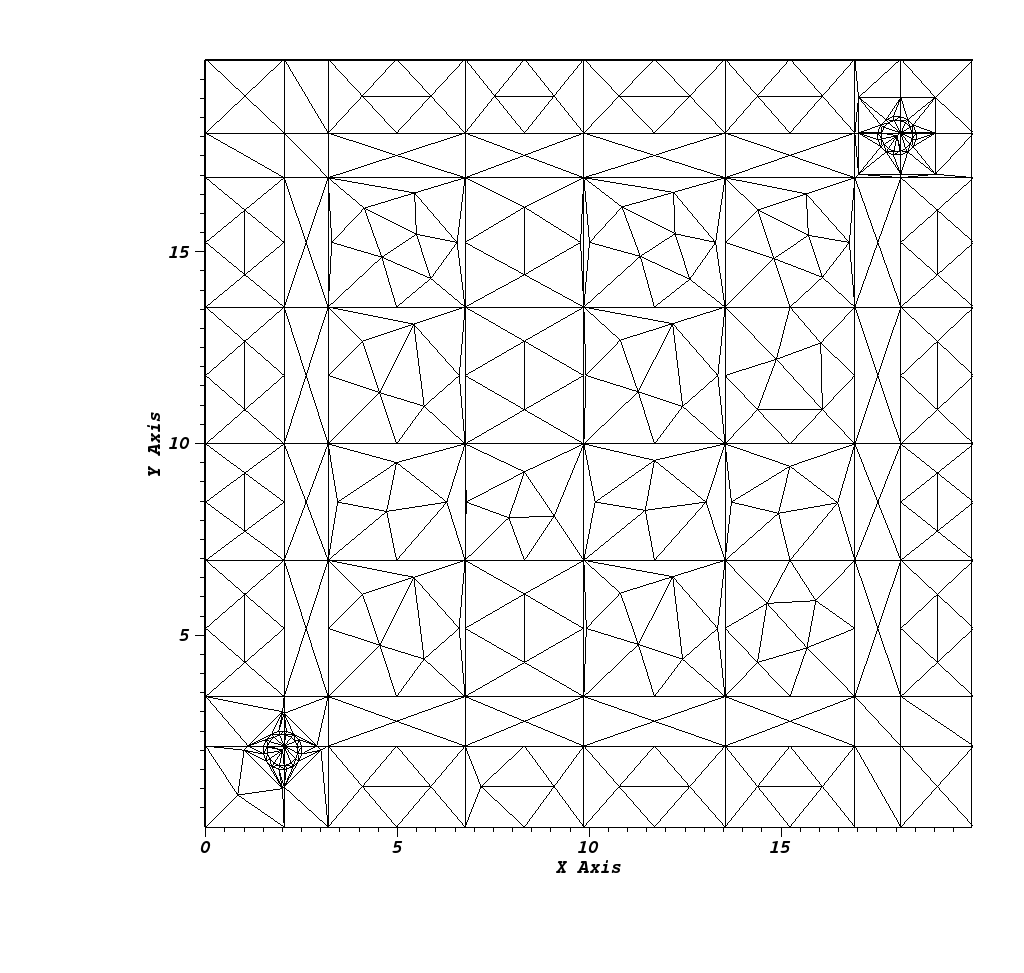
\includegraphics[scale = 0.22]{figures/redistribute_after.png}
\end{minipage}
\end{frame}

\section{Load Balancing Results}
%\subsection{}
\begin{frame}[t]\frametitle{Load Balancing Results}
\begin{block}{}
\begin{itemize}
	\item Three test cases were used to study the behavior of the load balancing algorithm.
	\item For each test case, 162 inputs were constructed by varying:
		\begin{itemize}
		\item The number of subsets
		\item The spatial resolution of the mesh (maximum triangle area).
		\end{itemize}
\end{itemize}
\end{block}
\end{frame}

\begin{frame}[t]\frametitle{Test Case 1}
\centering
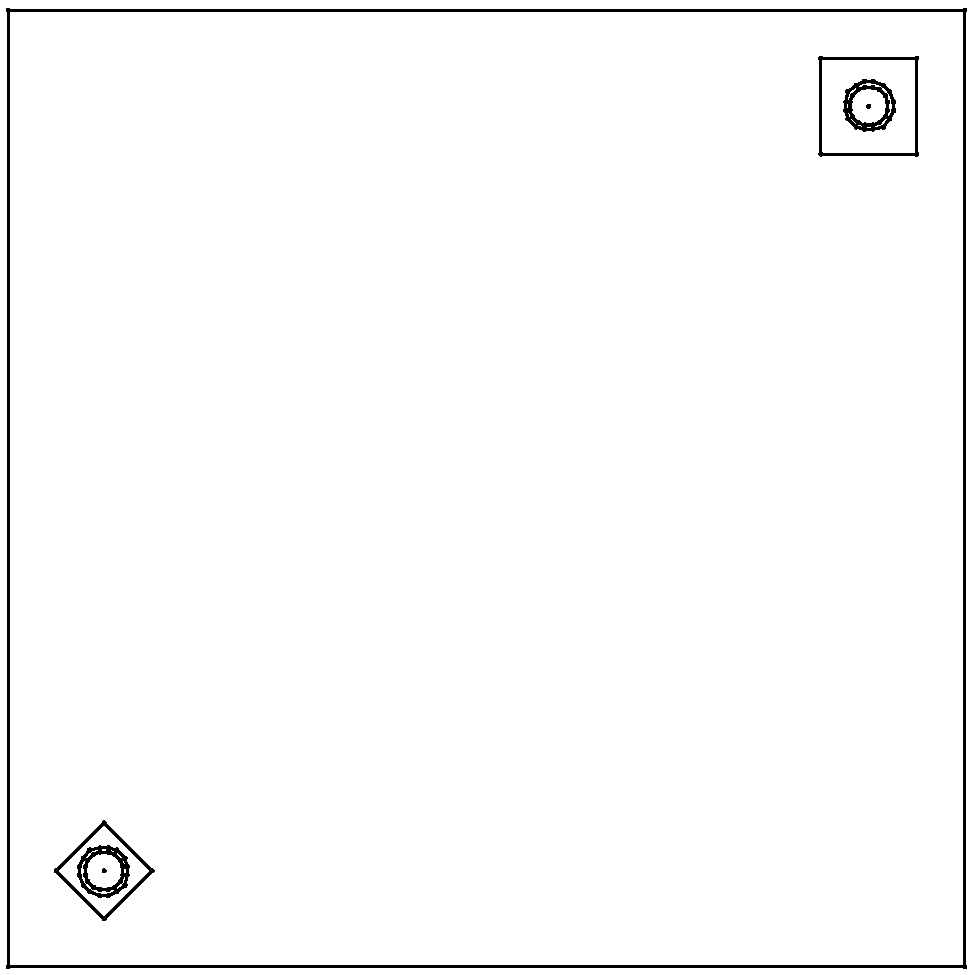
\includegraphics[scale = 0.4]{figures/unbalanced_lattice-eps-converted-to.pdf}
\end{frame}

%Tabulated case 1, No Iterations
\begin{frame}[t]\frametitle{Test Case 1}
\begin{table}[H]
\tiny
\centering
\caption{The metric behavior of the first test case run with \textbf{no load balancing} iterations.}
\begin{tabular}{rlrrrrrrrrr}
  \hline
 Area & N=4 & N=9 & N=16 & N=25 & N=36 & N=49 & N=64 & N=81 & N=100 \\ 
  \hline
 Coarse & 1.95 & 4.12 & 6.76 & 9.60 & 12.44 & 14.21 & 16.44 & 8.60 & 6.77 \\ 
   1.8 & 1.46 & 2.32 & 4.11 & 4.64 & 7.84 & 8.61 & \textbf{\cellcolor{blue!25}24.77} & 6.14 & 4.58 \\ 
 1.6 & 1.42 & 2.21 & 4.20 & 4.64 & 6.86 & 8.52 & 24.71 & 5.94 & 4.58 \\ 
 1.4 & 1.32 & 2.05 & 2.98 & 4.64 & 6.23 & 8.58 & 19.98 & 5.90 & 4.51 \\ 
 1.2 & 1.30 & 1.95 & 3.02 & 4.93 & 4.51 & 7.25 & 19.97 & 4.30 & 4.51 \\ 
  1 & 1.35 & 1.75 & 2.90 & 4.93 & 4.52 & 6.02 & 20.01 & 4.62 & 4.51 \\ 
  0.8 & 1.26 & 1.65 & 2.95 & 3.31 & 4.45 & 4.40 & 19.74 & 4.58 & 2.92 \\ 
   0.6 & 1.14 & 1.45 & 2.05 & 3.01 & 3.55 & 4.22 & 14.28 & 2.87 & 3.10 \\ 
 0.4 & 1.09 & 1.35 & 1.79 & 2.02 & 2.74 & 3.33 & 14.09 & 2.80 & 2.06 \\ 
   0.2 & 1.05 & 1.14 & 1.34 & 1.55 & 1.65 & 2.05 & 8.78 & 1.82 & 1.45 \\ 
  0.1 & 1.02 & 1.04 & 1.11 & 1.17 & 1.29 & 1.36 & 4.43 & 1.41 & 1.24 \\ 
  0.08 & 1.01 & 1.03 & 1.09 & 1.19 & 1.21 & 1.29 & 3.39 & 1.32 & 1.18 \\ 
 0.06 & 1.01 & 1.03 & 1.04 & 1.10 & 1.09 & 1.20 & 2.93 & 1.28 & 1.06 \\ 
  0.05 & 1.02 & 1.02 & 1.06 & 1.09 & 1.08 & 1.11 & 2.61 & 1.22 & 1.09 \\ 
   0.04 & 1.00 & 1.01 & 1.00 & 1.06 & 1.07 & 1.07 & 2.20 & 1.17 & 1.11 \\ 
  0.03 & 1.00 & 1.02 & 1.02 & 1.05 & 1.07 & 1.05 & 1.93 & 1.13 & 1.03 \\ 
   0.02 & 1.00 & 1.01 & 1.01 & 1.03 & 1.02 & 1.03 & 1.57 & 1.08 & 1.05 \\ 
  0.01 & \textbf{\cellcolor{blue!25}1.00} & 1.01 & 1.01 & 1.01 & 1.04 & 1.02 & 1.28 & 1.04 & 1.01 \\ 
   \hline
\end{tabular}
\end{table}
\end{frame}

%Tabulate iterations
\begin{frame}[t]\frametitle{Test Case 1}
\begin{table}[H]
\tiny
\centering
\caption{The metric behavior of the first test case after \textbf{10 load balancing iterations}.} 
\begin{tabular}{rlrrrrrrrrr}
  \hline
 Area & N=4 & N=9 & N=16 & N=25 & N=36 & N=49 & N=64 & N=81 & N=100 \\ 
  \hline
 Coarse & 1.95 & 1.60 & 3.37 & 2.10 & 2.28 & 2.68 & 2.53 & 2.81 & 3.05 \\ 
 1.8 & 1.46 & 1.94 & 2.81 & 2.59 & 2.98 & 2.89 & 2.97 & 4.50 & 4.33 \\ 
 1.6 & 1.42 & 1.95 & 2.43 & 2.42 & 3.00 & 3.05 & 2.71 & 4.11 & 4.09 \\ 
1.4 & 1.32 & 1.87 & 2.65 & 3.13 & 2.45 & 3.03 & 4.14 & 4.39 & 4.15 \\ 
 1.2 & 1.30 & 1.77 & 2.46 & 2.66 & 2.59 & 3.18 & 4.02 & 4.28 & \textbf{\cellcolor{blue!25}5.05} \\ 
  1 & 1.35 & 1.64 & 2.26 & 2.33 & 2.35 & 3.01 & 3.93 & 3.67 & 4.34 \\ 
 0.8 & 1.26 & 1.51 & 2.02 & 2.79 & 2.02 & 2.61 & 3.27 & 3.37 & 3.63 \\ 
 0.6 & 1.14 & 1.45 & 1.79 & 2.41 & 2.81 & 2.09 & 2.90 & 2.87 & 3.63 \\ 
   0.4 & 1.09 & 1.35 & 1.45 & 1.87 & 2.40 & 1.84 & 1.96 & 2.35 & 2.26 \\ 
   0.2 & 1.05 & 1.14 & 1.34 & 1.55 & 1.65 & 2.05 & 1.40 & 1.79 & 1.71 \\ 
  0.1 & 1.02 & 1.04 & 1.11 & 1.17 & 1.29 & 1.36 & 1.32 & 1.41 & 1.22 \\ 
  0.08 & 1.01 & 1.03 & 1.09 & 1.19 & 1.21 & 1.29 & 1.20 & 1.32 & 1.38 \\ 
   0.06 & 1.01 & 1.03 & 1.04 & 1.10 & 1.09 & 1.20 & 1.15 & 1.28 & 1.07 \\ 
   0.05 & 1.02 & 1.02 & 1.06 & 1.09 & 1.08 & 1.11 & 1.14 & 1.22 & 1.18 \\ 
   0.04 & 1.00 & 1.01 & 1.00 & 1.06 & 1.07 & 1.07 & 1.16 & 1.17 & 1.17 \\ 
   0.03 & 1.00 & 1.02 & 1.02 & 1.05 & 1.07 & 1.05 & 1.93 & 1.13 & 1.04 \\ 
   0.02 & 1.00 & 1.01 & 1.01 & 1.03 & 1.02 & 1.03 & 1.57 & 1.08 & 1.09 \\ 
   0.01 & \textbf{\cellcolor{blue!25}1.00} & 1.01 & 1.01 & 1.01 & 1.04 & 1.02 & 1.28 & 1.04 & 1.02 \\ 
   \hline
\end{tabular}
\end{table}
\end{frame}



%Table Diff
\begin{frame}\frametitle{Test Case 1}
\begin{table}[H]
\tiny
\centering
\caption{The ratio  of the metric with no iteration and 10 iterations. The closer the z-value to zero, the better the improvement.} 
\begin{tabular}{rlrrrrrrrrr}
  \hline
 Area & N=4 & N=9 & N=16 & N=25 & N=36 & N=49 & N=64 & N=81 & N=100 \\ 
  \hline
 Coarse & 1.00 & 0.39 & 0.50 & 0.22 & 0.18 & 0.19 & 0.15 & 0.33 & 0.45 \\ 
   1.8 & 1.00 & 0.83 & 0.68 & 0.56 & 0.38 & 0.34 & 0.12 & 0.73 & 0.95 \\ 
   1.6 & 1.00 & 0.88 & 0.58 & 0.52 & 0.44 & 0.36 & \textbf{\cellcolor{blue!25}0.11} & 0.69 & 0.89 \\ 
  1.4 & 1.00 & 0.91 & 0.89 & 0.67 & 0.39 & 0.35 & 0.21 & 0.74 & 0.92 \\ 
   1.2 & 1.00 & 0.90 & 0.81 & 0.54 & 0.58 & 0.44 & 0.20 & 1.00 & 1.12 \\ 
   1 & 1.00 & 0.93 & 0.78 & 0.47 & 0.52 & 0.50 & 0.20 & 0.79 & 0.96 \\ 
0.8 & 1.00 & 0.92 & 0.68 & 0.84 & 0.45 & 0.59 & 0.17 & 0.74 & \textbf{\cellcolor{blue!25}1.24} \\ 
  0.6 & 1.00 & 1.00 & 0.87 & 0.80 & 0.79 & 0.50 & 0.20 & 1.00 & 1.17 \\ 
 0.4 & 1.00 & 1.00 & 0.81 & 0.93 & 0.88 & 0.55 & 0.14 & 0.84 & 1.10 \\ 
  0.2 & 1.00 & 1.00 & 1.00 & 1.00 & 1.00 & 1.00 & 0.16 & 0.99 & 1.19 \\ 
  0.1 & 1.00 & 1.00 & 1.00 & 1.00 & 1.00 & 1.00 & 0.30 & 1.00 & 0.98 \\ 
   0.08 & 1.00 & 1.00 & 1.00 & 1.00 & 1.00 & 1.00 & 0.35 & 1.00 & 1.17 \\ 
   0.06 & 1.00 & 1.00 & 1.00 & 1.00 & 1.00 & 1.00 & 0.39 & 1.00 & 1.00 \\ 
   0.05 & 1.00 & 1.00 & 1.00 & 1.00 & 1.00 & 1.00 & 0.44 & 1.00 & 1.08 \\ 
   0.04 & 1.00 & 1.00 & 1.00 & 1.00 & 1.00 & 1.00 & 0.52 & 1.00 & 1.05 \\ 
   0.03 & 1.00 & 1.00 & 1.00 & 1.00 & 1.00 & 1.00 & 1.00 & 1.00 & 1.01 \\ 
  0.02 & 1.00 & 1.00 & 1.00 & 1.00 & 1.00 & 1.00 & 1.00 & 1.00 & 1.04 \\ 
   0.01 & 1.00 & 1.00 & 1.00 & 1.00 & 1.00 & 1.00 & 1.00 & 1.00 & 1.01 \\ 
   \hline
\end{tabular}
\end{table}
\end{frame}

\begin{frame}[t]\frametitle{Test Case 2}
\centering
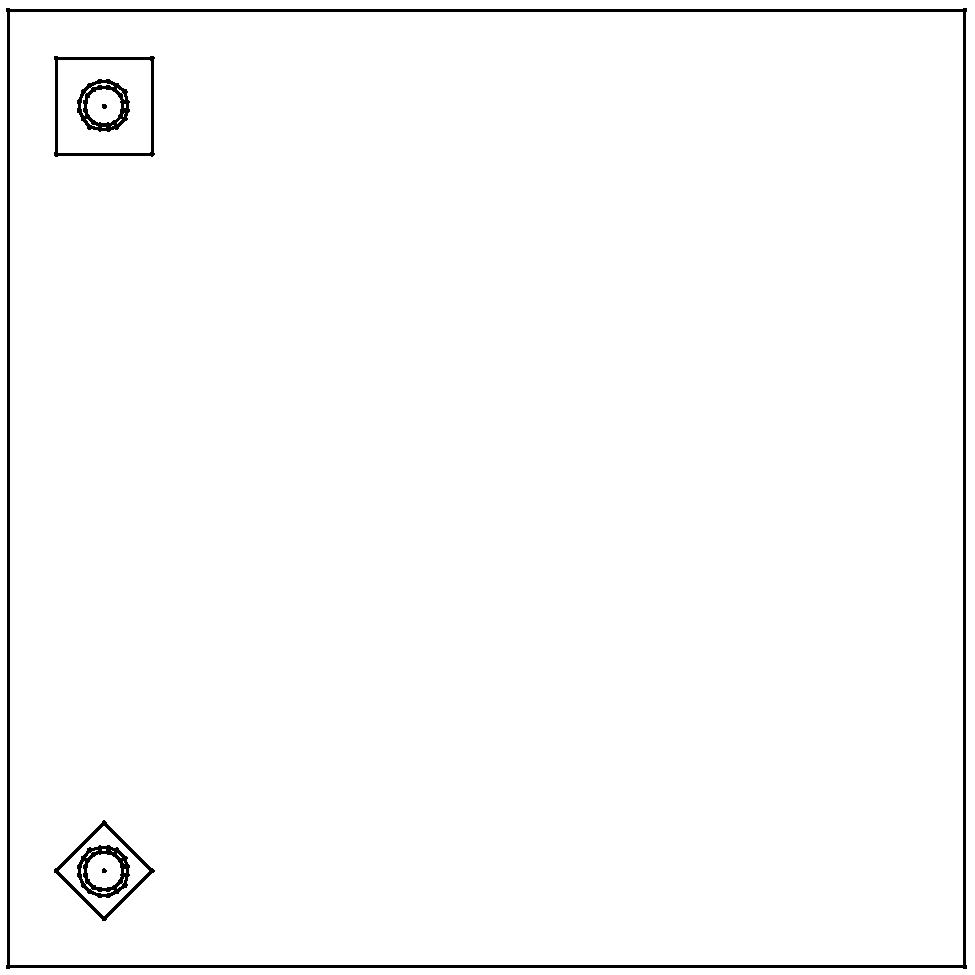
\includegraphics[scale = 0.4]{figures/unbalanced_pins_same_side-eps-converted-to.pdf}
\end{frame}

%Test Case 2 no iter
\begin{frame}[t]\frametitle{Test Case 2}
\begin{table}[H]
\tiny
\centering
\caption{The metric behavior of the second test case after \textbf{no load balancing} iterations.} 
\begin{tabular}{rrrrrrrrrrr}
  \hline
 Area & N=4 & N=9 & N=16 & N=25 & N=36 & N=49 & N=64 & N=81 & N=100 \\ 
  \hline
 Coarse & 1.95 & 4.12 & 6.76 & 9.60 & 12.44 & 14.21 & 16.44 & 8.60 & 6.77 \\ 
1.80 & 1.45 & 2.31 & 4.10 & 4.91 & 7.90 & 8.61 & \textbf{\cellcolor{blue!25}22.67} & 6.37 & 6.19 \\ 
 1.60 & 1.42 & 2.24 & 4.19 & 4.91 & 6.94 & 8.50 & 20.91 & 6.29 & 6.19 \\ 
 1.40 & 1.31 & 2.12 & 2.97 & 4.41 & 6.22 & 8.58 & 19.84 & 6.25 & 5.99 \\ 
 1.20 & 1.30 & 1.96 & 3.02 & 4.65 & 4.53 & 7.09 & 19.83 & 4.30 & 6.23 \\ 
 1.00 & 1.34 & 1.78 & 2.90 & 4.35 & 4.49 & 5.88 & 19.85 & 4.62 & 4.98 \\ 
 0.80 & 1.26 & 1.64 & 2.95 & 3.09 & 4.47 & 4.45 & 17.42 & 4.58 & 4.18 \\ 
  0.60 & 1.14 & 1.42 & 2.05 & 2.72 & 3.50 & 4.09 & 12.90 & 2.80 & 4.18 \\ 
 0.40 & 1.09 & 1.34 & 1.79 & 2.08 & 2.73 & 3.34 & 11.39 & 2.83 & 2.68 \\ 
 0.20 & 1.06 & 1.15 & 1.34 & 1.56 & 1.72 & 2.03 & 7.02 & 1.85 & 1.72 \\ 
  0.10 & 1.02 & 1.04 & 1.15 & 1.22 & 1.29 & 1.37 & 4.12 & 1.36 & 1.37 \\ 
   0.08 & 1.01 & 1.04 & 1.08 & 1.15 & 1.20 & 1.30 & 3.47 & 1.33 & 1.26 \\ 
  0.06 & 1.01 & 1.03 & 1.04 & 1.10 & 1.08 & 1.20 & 2.79 & 1.26 & 1.19 \\ 
 0.05 & 1.02 & 1.03 & 1.05 & 1.07 & 1.06 & 1.12 & 2.57 & 1.23 & 1.16 \\ 
 0.04 & 1.00 & 1.03 & 1.01 & 1.06 & 1.08 & 1.07 & 2.22 & 1.18 & 1.11 \\ 
 0.03 & 1.01 & 1.02 & 1.01 & 1.04 & 1.07 & 1.05 & 1.86 & 1.11 & 1.08 \\ 
  0.02 & 1.01 & 1.02 & 1.01 & 1.04 & 1.04 & 1.03 & 1.57 & 1.09 & 1.07 \\ 
 0.01 & \textbf{\cellcolor{blue!25}1.00} & 1.01 & 1.02 & 1.02 & 1.02 & 1.02 & 1.29 & 1.04 & 1.02 \\ 
   \hline
\end{tabular}
\end{table}
\end{frame}

\begin{frame}[t]\frametitle{Test Case 2}
\begin{table}[H]
\centering
\tiny
\caption{The metric behavior of the second test case after \textbf{10 load balancing iterations}.} 
\begin{tabular}{rlrrrrrrrrr}
  \hline
 Area & N=4 & N=9 & N=16 & N=25 & N=36 & N=49 & N=64 & N=81 & N=100 \\ 
  \hline
 Coarse & 1.85 & 1.36 & 1.76 & 1.48 & 1.74 & 1.60 & 1.79 & 1.82 & 1.92 \\ 
   1.8 & 1.15 & 1.33 & 1.65 & 2.08 & 2.58 & 2.41 & 2.69 & 3.83 & \textbf{\cellcolor{blue!25}3.99} \\ 
 1.6 & 1.12 & 1.34 & 1.65 & 2.35 & 2.67 & 2.47 & 2.96 & 2.59 & 2.97 \\ 
1.4 & 1.12 & 1.37 & 1.79 & 1.86 & 1.83 & 2.71 & 2.82 & 2.58 & 3.74 \\ 
 1.2 & 1.15 & 1.50 & 1.54 & 1.56 & 1.71 & 2.13 & 2.81 & 2.79 & 2.87 \\ 
 1 & 1.15 & 1.45 & 1.73 & 1.74 & 1.74 & 2.39 & 2.48 & 2.81 & 3.07 \\ 
0.8 & 1.14 & 1.40 & 1.47 & 1.44 & 1.58 & 2.26 & 2.38 & 2.60 & 3.39 \\ 
 0.6 & 1.05 & 1.31 & 1.49 & 1.85 & 1.57 & 1.81 & 1.81 & 2.42 & 2.36 \\ 
 0.4 & 1.09 & 1.19 & 1.37 & 1.77 & 1.71 & 1.87 & 1.57 & 1.72 & 2.26 \\ 
 0.2 & 1.06 & 1.15 & 1.18 & 1.35 & 1.63 & 1.67 & 1.73 & 1.52 & 1.72 \\ 
 0.1 & 1.02 & 1.04 & 1.15 & 1.22 & 1.29 & 1.34 & 1.25 & 1.26 & 1.37 \\ 
   0.08 & 1.01 & 1.04 & 1.08 & 1.15 & 1.20 & 1.30 & 1.22 & 1.21 & 1.26 \\ 
0.06 & 1.01 & 1.03 & 1.04 & 1.10 & 1.08 & 1.20 & 1.18 & 1.26 & 1.19 \\ 
   0.05 & 1.02 & 1.03 & 1.05 & 1.07 & 1.06 & 1.12 & 1.15 & 1.23 & 1.16 \\ 
  0.04 & 1.00 & 1.03 & 1.01 & 1.06 & 1.08 & 1.07 & 1.13 & 1.18 & 1.11 \\ 
 0.03 & 1.01 & 1.02 & 1.01 & 1.04 & 1.07 & 1.05 & 1.32 & 1.11 & 1.08 \\ 
  0.02 & 1.01 & 1.02 & 1.01 & 1.04 & 1.04 & 1.03 & 1.15 & 1.09 & 1.07 \\ 
 0.01 & \textbf{\cellcolor{blue!25}1.00} & 1.01 & 1.02 & 1.02 & 1.02 & 1.02 & 1.29 & 1.04 & 1.02 \\ 
   \hline
\end{tabular}
\end{table}
\end{frame}

%Test Case 2 Improvement
\begin{frame}[t]\frametitle{Test Case 2}
\begin{table}[H]
\centering
\tiny
\caption{The ratio  of the metric with no iteration and 10 iterations. The closer the z-value to zero, the better the improvement.} 
\begin{tabular}{rlrrrrrrrrr}
  \hline
  Area & N=4 & N=9 & N=16 & N=25 & N=36 & N=49 & N=64 & N=81 & N=100 \\ 
  \hline
Coarse & 0.95 & 0.33 & 0.26 & 0.15 & 0.14 & 0.11 & \textbf{\cellcolor{blue!25}0.11} & 0.21 & 0.28 \\ 
  1.8 & 0.79 & 0.57 & 0.40 & 0.42 & 0.33 & 0.28 & 0.12 & 0.60 & 0.65 \\ 
1.6 & 0.79 & 0.60 & 0.39 & 0.48 & 0.38 & 0.29 & 0.14 & 0.41 & 0.48 \\ 
 1.4 & 0.85 & 0.64 & 0.60 & 0.42 & 0.29 & 0.32 & 0.14 & 0.41 & 0.62 \\ 
 1.2 & 0.89 & 0.77 & 0.51 & 0.34 & 0.38 & 0.30 & 0.14 & 0.65 & 0.46 \\ 
 1 & 0.85 & 0.81 & 0.60 & 0.40 & 0.39 & 0.41 & 0.12 & 0.61 & 0.62 \\ 
  0.8 & 0.91 & 0.85 & 0.50 & 0.47 & 0.35 & 0.51 & 0.14 & 0.57 & 0.81 \\ 
 0.6 & 0.92 & 0.92 & 0.73 & 0.68 & 0.45 & 0.44 & 0.14 & 0.86 & 0.57 \\ 
 0.4 & 1.00 & 0.89 & 0.76 & 0.85 & 0.63 & 0.56 & 0.14 & 0.61 & 0.84 \\ 
   0.2 & 1.00 & 1.00 & 0.89 & 0.86 & 0.95 & 0.82 & 0.25 & 0.82 & 1.00 \\ 
   0.1 & 1.00 & 1.00 & 1.00 & 1.00 & 1.00 & 0.98 & 0.30 & 0.92 & 1.00 \\ 
 0.08 & 1.00 & 1.00 & 1.00 & 1.00 & 1.00 & 1.00 & 0.35 & 0.91 & 1.00 \\ 
 0.06 & 1.00 & 1.00 & 1.00 & 1.00 & 1.00 & 1.00 & 0.42 & 1.00 & 1.00 \\ 
   0.05 & 1.00 & 1.00 & 1.00 & 1.00 & 1.00 & 1.00 & 0.45 & 1.00 & 1.00 \\ 
   0.04 & 1.00 & 1.00 & 1.00 & 1.00 & 1.00 & 1.00 & 0.51 & 1.00 & 1.00 \\ 
   0.03 & 1.00 & 1.00 & 1.00 & 1.00 & 1.00 & 1.00 & 0.71 & 1.00 & 1.00 \\ 
   0.02 & 1.00 & 1.00 & 1.00 & 1.00 & 1.00 & 1.00 & 0.74 & 1.00 & 1.00 \\ 
 0.01 & \textbf{\cellcolor{blue!25}1.00} & 1.00 & 1.00 & 1.00 & 1.00 & 1.00 & 1.00 & 1.00 & 1.00 \\ 
   \hline
\end{tabular}
\end{table}
\end{frame}

\begin{frame}[t]\frametitle{A Closer Look at Test Case 2}
\begin{minipage}{0.15\textwidth}
\begin{footnotesize}
Iter 0 \\
$f$ = 2.72
\end{footnotesize}
\end{minipage}
\begin{minipage}{0.8\textwidth}
\centering
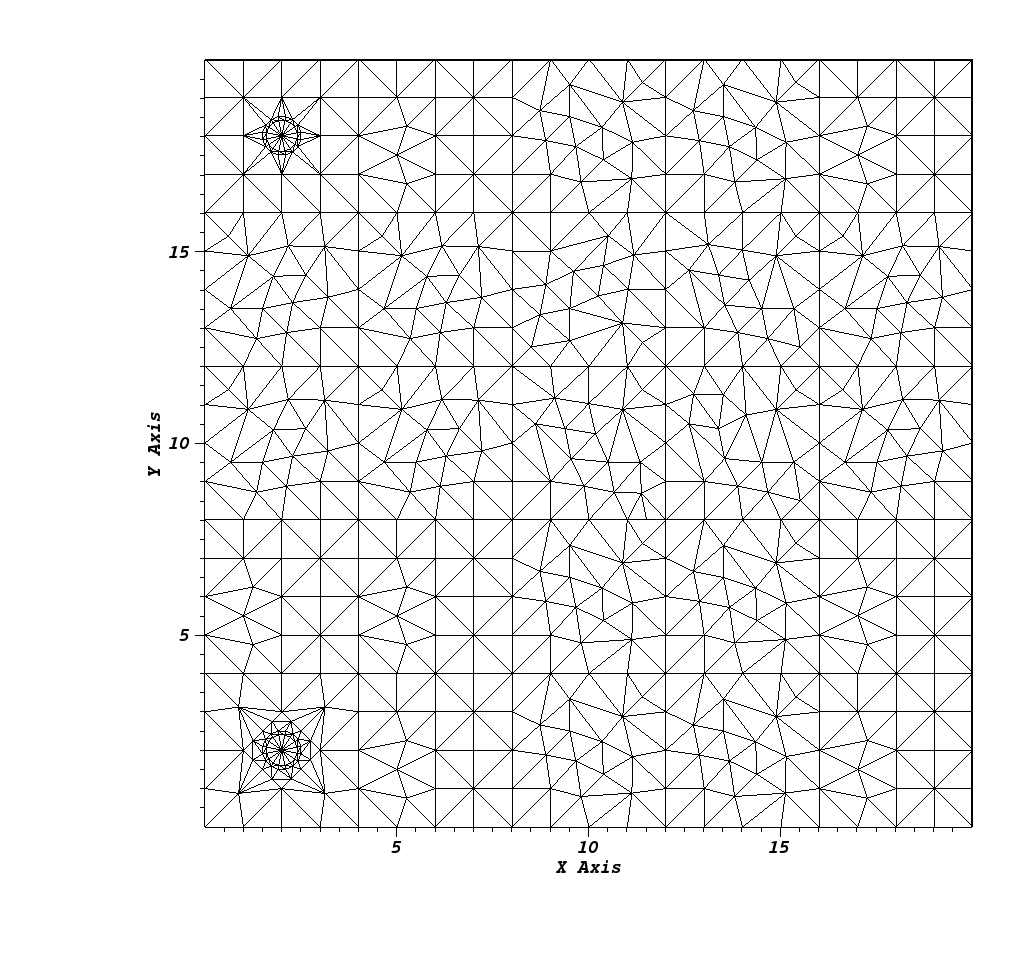
\includegraphics[scale=0.22]{figures/sameside_before.png}
\end{minipage}
\end{frame}

\begin{frame}[t]\frametitle{A Closer Look at Test Case 2}
\begin{minipage}{0.15\textwidth}
\begin{footnotesize}
Iter 10\\
$f$ =1.85
\end{footnotesize}
\end{minipage}
\begin{minipage}{0.8\textwidth}
\centering
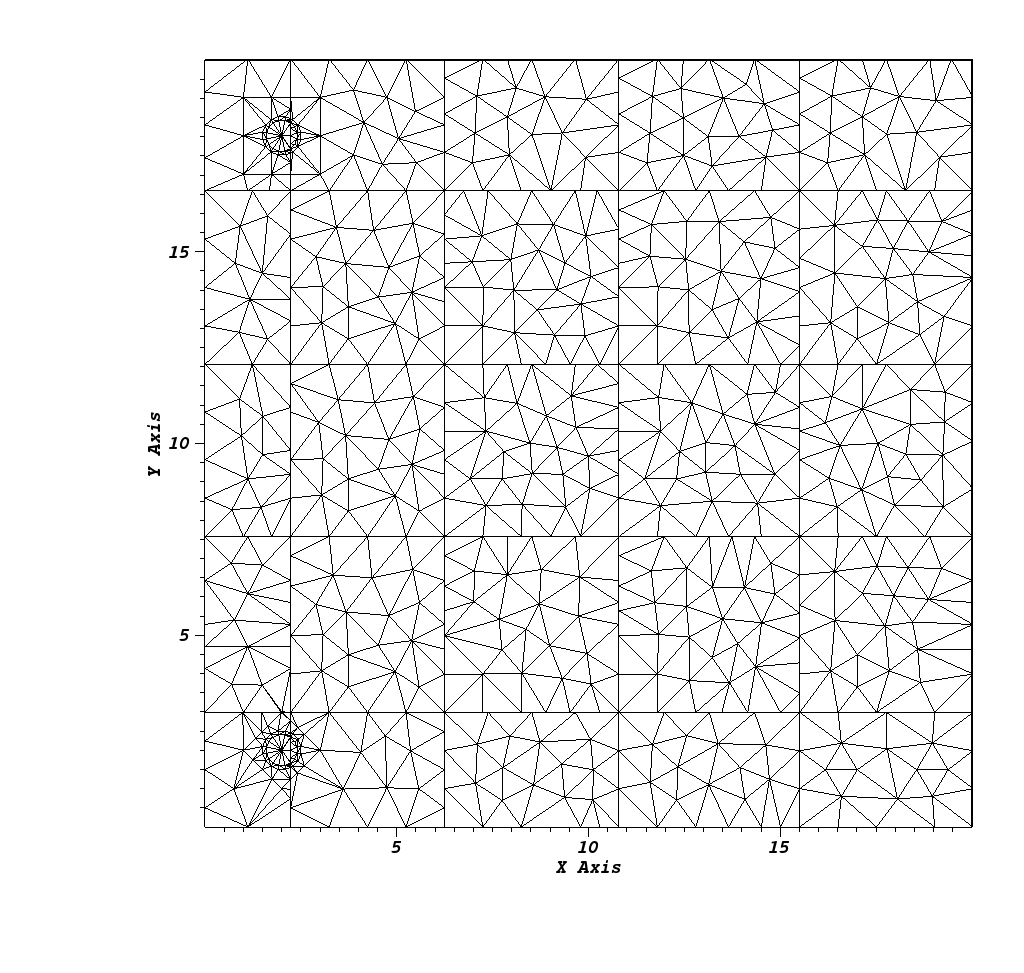
\includegraphics[scale=0.22]{figures/sameside_after.png}
\end{minipage}
\end{frame}

\begin{frame}[t]\frametitle{Test Case 3}
\centering
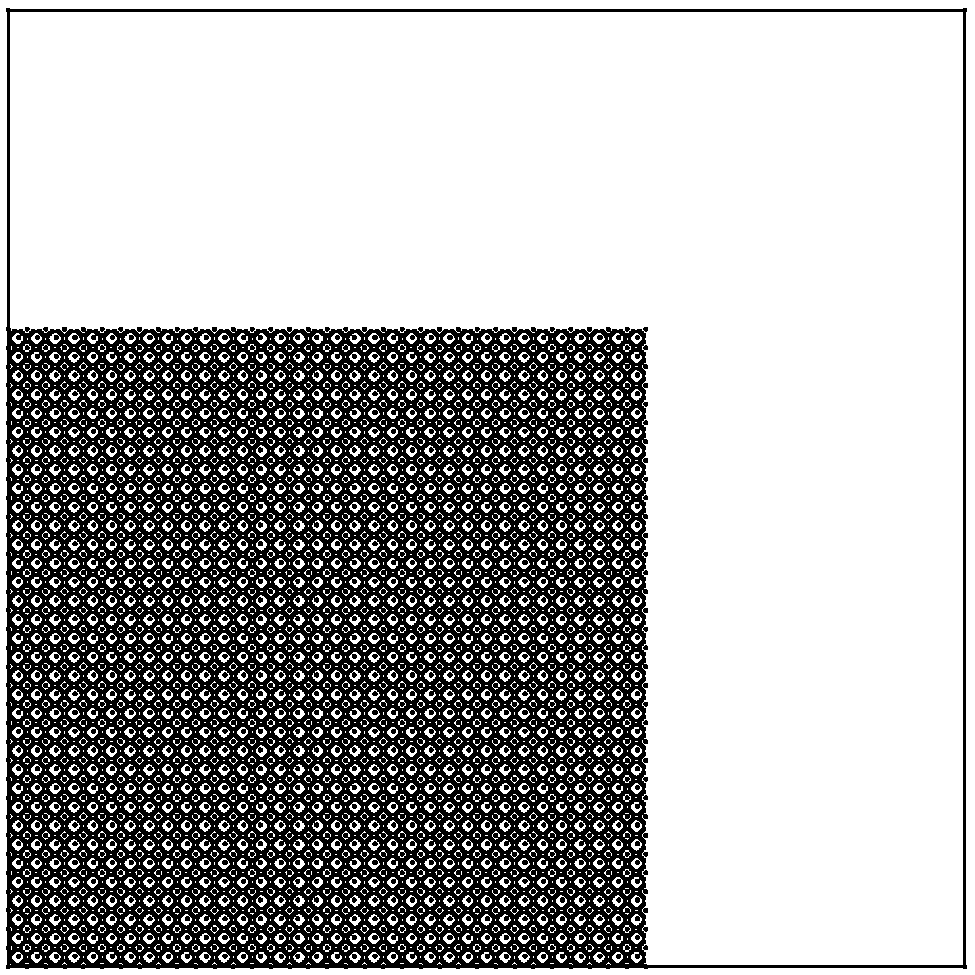
\includegraphics[scale = 0.4]{figures/lattice-12-shifted-eps-converted-to.pdf}
\end{frame}


%Test 3 no iter
\begin{frame}[t]\frametitle{Test Case 3}
\begin{table}[H]
\tiny
\centering
\caption{The metric behavior of the third test case after\textbf{ no load balancing iterations}.} 
\begin{tabular}{rlrrrrrrrrr}
  \hline
 Area & N=4 & N=9 & N=16 & N=25 & N=36 & N=49 & N=64 & N=81 & N=100 \\ 
  \hline
 Coarse & 2.24 & 2.24 & 2.28 & 2.27 & 2.24 & 2.29 & 2.32 & 2.26 & 2.29 \\ 
 1.8 & 2.13 & 2.13 & 2.16 & 2.42 & 2.13 & 2.43 & 2.23 & 2.17 & \textbf{\cellcolor{blue!25}2.65} \\ 
   1.6 & 2.11 & 2.12 & 2.15 & 2.40 & 2.11 & 2.42 & 2.22 & 2.16 & 2.63 \\ 
   1.4 & 2.09 & 2.10 & 2.13 & 2.38 & 2.10 & 2.39 & 2.20 & 2.12 & 2.61 \\ 
 1.2 & 2.07 & 2.07 & 2.11 & 2.35 & 2.08 & 2.37 & 2.18 & 2.11 & 2.59 \\ 
 1 & 2.04 & 2.04 & 2.07 & 2.32 & 2.04 & 2.33 & 2.15 & 2.08 & 2.54 \\ 
 0.8 & 1.99 & 1.99 & 2.02 & 2.27 & 1.99 & 2.28 & 2.10 & 2.03 & 2.50 \\ 
0.6 & 1.91 & 1.92 & 1.95 & 2.18 & 1.92 & 2.20 & 2.03 & 1.96 & 2.41 \\ 
 0.4 & 1.78 & 1.79 & 1.82 & 2.04 & 1.79 & 2.06 & 1.90 & 1.83 & 2.27 \\ 
 0.2 & 1.47 & 1.48 & 1.51 & 1.70 & 1.49 & 1.72 & 1.59 & 1.52 & 1.91 \\ 
   0.1 & 1.09 & 1.10 & 1.12 & 1.28 & 1.11 & 1.29 & 1.21 & 1.16 & 1.45 \\ 
 0.08 & 1.03 & 1.02 & 1.03 & 1.13 & 1.02 & 1.15 & 1.07 & 1.03 & 1.31 \\ 
 0.06 & 1.03 & 1.04 & 1.04 & 1.15 & 1.04 & 1.18 & 1.09 & 1.08 & 1.28 \\ 
0.05 & 1.02 & 1.02 & 1.03 & 1.11 & 1.03 & 1.13 & 1.09 & 1.06 & 1.20 \\ 
 0.04 & 1.06 & 1.06 & 1.06 & 1.12 & 1.08 & 1.12 & 1.09 & 1.10 & 1.20 \\ 
  0.03 & 1.08 & 1.08 & 1.09 & 1.12 & 1.10 & 1.11 & 1.10 & 1.11 & 1.15 \\ 
  0.02 & \textbf{\cellcolor{blue!25}1.02} & 1.03 & 1.03 & 1.03 & 1.03 & 1.03 & 1.03 & 1.03 & 1.06 \\ 
 0.01 & 1.03 & 1.03 & 1.03 & 1.04 & 1.03 & 1.04 & 1.04 & 1.03 & 1.05 \\ 
   \hline
\end{tabular}
\end{table}
\end{frame}


%Test Case 3 iter
\begin{frame}[t]\frametitle{Test Case 3}
\begin{table}[H]
\tiny
\centering
\caption{The metric behavior of the third test case after \textbf{10 load balancing iterations}.} 
\begin{tabular}{rlrrrrrrrrr}
  \hline
  Area & N=4 & N=9 & N=16 & N=25 & N=36 & N=49 & N=64 & N=81 & N=100 \\ 
  \hline
 Coarse & \textbf{\cellcolor{blue!25}1.00} & 1.01 & 1.04 & 1.05 & 1.01 & 1.06 & 1.06 & 1.06 & 1.08 \\ 
1.8 & 1.02 & 1.03 & 1.15 & 1.21 & 1.20 & 1.23 & 1.36 & 1.42 & 1.54 \\ 
  1.6 & 1.03 & 1.04 & 1.08 & 1.20 & 1.18 & 1.23 & 1.54 & 1.69 & 1.58 \\ 
1.4 & 1.02 & 1.06 & 1.09 & 1.25 & 1.32 & 1.39 & 1.37 & 1.52 & 1.62 \\ 
 1.2 & 1.03 & 1.06 & 1.24 & 1.24 & 1.30 & 1.32 & 1.48 & 1.56 & 1.84 \\ 
 1 & 1.02 & 1.05 & 1.15 & 1.25 & 1.31 & 1.35 & 1.49 & 1.80 & 2.15 \\ 
 0.8 & 1.04 & 1.06 & 1.10 & 1.23 & 1.27 & 1.53 & 1.79 & 1.84 & 1.95 \\ 
 0.6 & 1.03 & 1.11 & 1.13 & 1.38 & 1.51 & 1.61 & 1.79 & 1.96 & 2.17 \\ 
   0.4 & 1.04 & 1.19 & 1.26 & 1.39 & 1.66 & 1.47 & 1.90 & 1.83 & \textbf{\cellcolor{blue!25}2.27} \\ 
   0.2 & 1.06 & 1.17 & 1.16 & 1.33 & 1.49 & 1.62 & 1.59 & 1.52 & 1.78 \\ 
 0.1 & 1.09 & 1.10 & 1.12 & 1.14 & 1.11 & 1.19 & 1.21 & 1.16 & 1.19 \\ 
 0.08 & 1.03 & 1.02 & 1.03 & 1.13 & 1.02 & 1.15 & 1.07 & 1.03 & 1.14 \\ 
  0.06 & 1.03 & 1.04 & 1.04 & 1.15 & 1.04 & 1.18 & 1.09 & 1.08 & 1.28 \\ 
   0.05 & 1.02 & 1.02 & 1.03 & 1.11 & 1.03 & 1.13 & 1.09 & 1.06 & 1.20 \\ 
   0.04 & 1.06 & 1.06 & 1.06 & 1.12 & 1.08 & 1.12 & 1.09 & 1.10 & 1.20 \\ 
 0.03 & 1.08 & 1.08 & 1.09 & 1.12 & 1.10 & 1.11 & 1.10 & 1.11 & 1.15 \\ 
0.02 & 1.02 & 1.03 & 1.03 & 1.03 & 1.03 & 1.03 & 1.03 & 1.03 & 1.06 \\ 
 0.01 & 1.03 & 1.03 & 1.03 & 1.04 & 1.03 & 1.04 & 1.04 & 1.03 & 1.05 \\ 
   \hline
\end{tabular}
\end{table}
\end{frame}

%Test Case Diff
\begin{frame}[t]\frametitle{Test Case 3}
\begin{table}[H]
\centering
\tiny
\caption{The ratio  of the metric with no iteration and 10 iterations. The closer the z-value to zero, the better the improvement.} 
\begin{tabular}{rlrrrrrrrrr}
  \hline
  Area & N=4 & N=9 & N=16 & N=25 & N=36 & N=49 & N=64 & N=81 & N=100 \\ 
  \hline
Coarse & \textbf{\cellcolor{blue!25}0.45} & 0.45 & 0.46 & 0.46 & 0.45 & 0.46 & 0.45 & 0.47 & 0.47 \\ 
  1.8 & 0.48 & 0.48 & 0.53 & 0.50 & 0.56 & 0.51 & 0.61 & 0.65 & 0.58 \\ 
 1.6 & 0.49 & 0.49 & 0.50 & 0.50 & 0.56 & 0.51 & 0.69 & 0.78 & 0.60 \\ 
 1.4 & 0.49 & 0.50 & 0.51 & 0.52 & 0.63 & 0.58 & 0.62 & 0.72 & 0.62 \\ 
 1.2 & 0.50 & 0.51 & 0.59 & 0.53 & 0.62 & 0.56 & 0.68 & 0.74 & 0.71 \\ 
1 & 0.50 & 0.51 & 0.56 & 0.54 & 0.64 & 0.58 & 0.69 & 0.86 & 0.85 \\ 
 0.8 & 0.52 & 0.53 & 0.54 & 0.54 & 0.64 & 0.67 & 0.85 & 0.90 & 0.78 \\ 
 0.6 & 0.54 & 0.58 & 0.58 & 0.63 & 0.79 & 0.73 & 0.88 & 1.00 & 0.90 \\ 
 0.4 & 0.59 & 0.66 & 0.70 & 0.68 & 0.93 & 0.71 & 1.00 & 1.00 & 1.00 \\ 
   0.2 & 0.72 & 0.79 & 0.77 & 0.78 & 1.00 & 0.94 & 1.00 & 1.00 & 0.93 \\ 
 0.1 & 1.00 & 1.00 & 1.00 & 0.89 & 1.00 & 0.92 & 1.00 & 1.00 & 0.83 \\ 
 0.08 & 1.00 & 1.00 & 1.00 & 1.00 & 1.00 & 1.00 & 1.00 & 1.00 & 0.87 \\ 
 0.06 & 1.00 & 1.00 & 1.00 & 1.00 & 1.00 & 1.00 & 1.00 & 1.00 & 1.00 \\ 
 0.05 & 1.00 & 1.00 & 1.00 & 1.00 & 1.00 & 1.00 & 1.00 & 1.00 & 1.00 \\ 
0.04 & 1.00 & 1.00 & 1.00 & 1.00 & 1.00 & 1.00 & 1.00 & 1.00 & 1.00 \\ 
  0.03 & 1.00 & 1.00 & 1.00 & 1.00 & 1.00 & 1.00 & 1.00 & 1.00 & 1.00 \\ 
  0.02 & 1.00 & 1.00 & 1.00 & 1.00 & 1.00 & 1.00 & 1.00 & 1.00 & 1.00 \\ 
  0.01 & \textbf{\cellcolor{blue!25}1.00} & 1.00 & 1.00 & 1.00 & 1.00 & 1.00 & 1.00 & 1.00 & 1.00 \\ 
   \hline
\end{tabular}
\end{table}
\end{frame}

\begin{frame}[t]\frametitle{IM1-B}
\centering
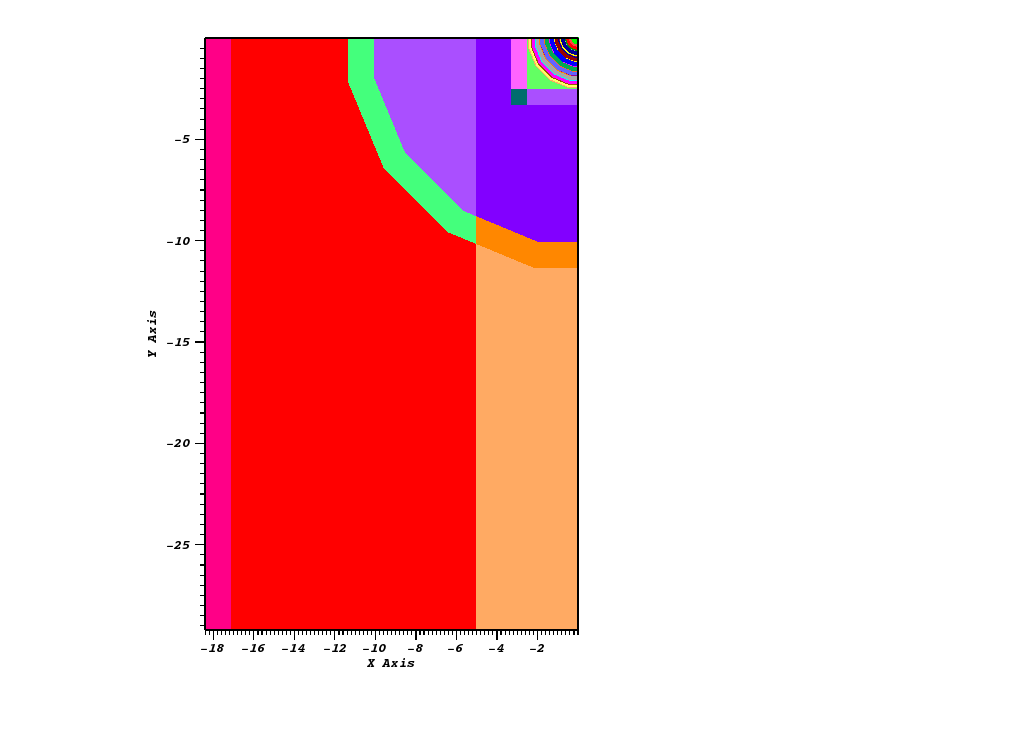
\includegraphics[scale = 0.3]{figures/IM1_filled_boundary0000.png}
\end{frame}

\begin{frame}[t]\frametitle{Iteration 0}
\begin{minipage}{0.15\textwidth}
\begin{footnotesize}
$f = 42.1526$
\end{footnotesize}
\end{minipage}
\begin{minipage}{0.8\textwidth}
\centering
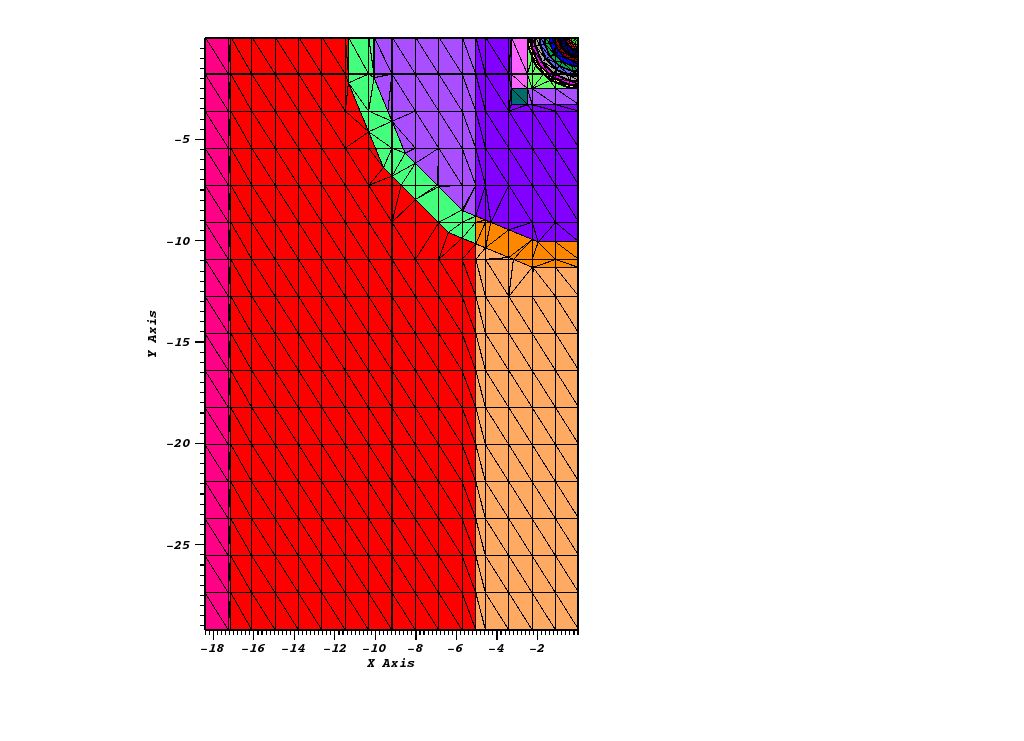
\includegraphics[scale=0.3]{figures/IM1_pre_iterations0000.png}
\end{minipage}
\end{frame}

\begin{frame}[t]\frametitle{Iteration 7}
\begin{minipage}{0.15\textwidth}
\begin{footnotesize}
$f = 2.99$
\end{footnotesize}
\end{minipage}
\begin{minipage}{0.8\textwidth}
\centering
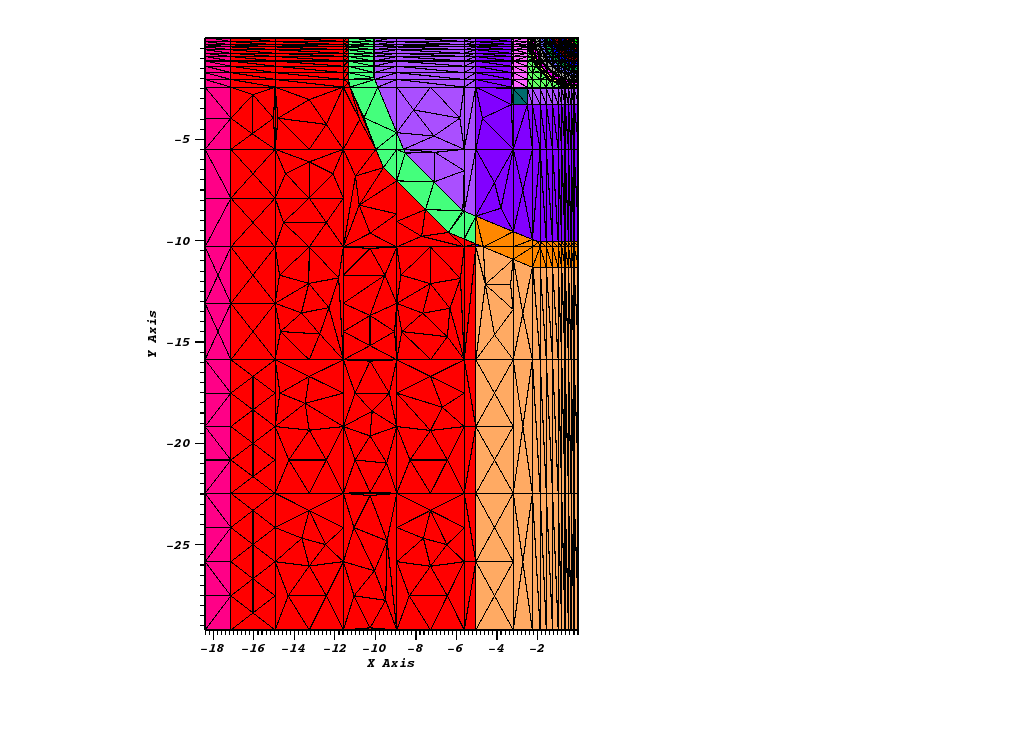
\includegraphics[scale=0.3]{figures/IM1_post_iterations0000.png}
\end{minipage}
\end{frame}


\section{Conclusions}
%\subsection{}

\begin{frame}[t]\frametitle{Extruded Mesh Capability}
\centering
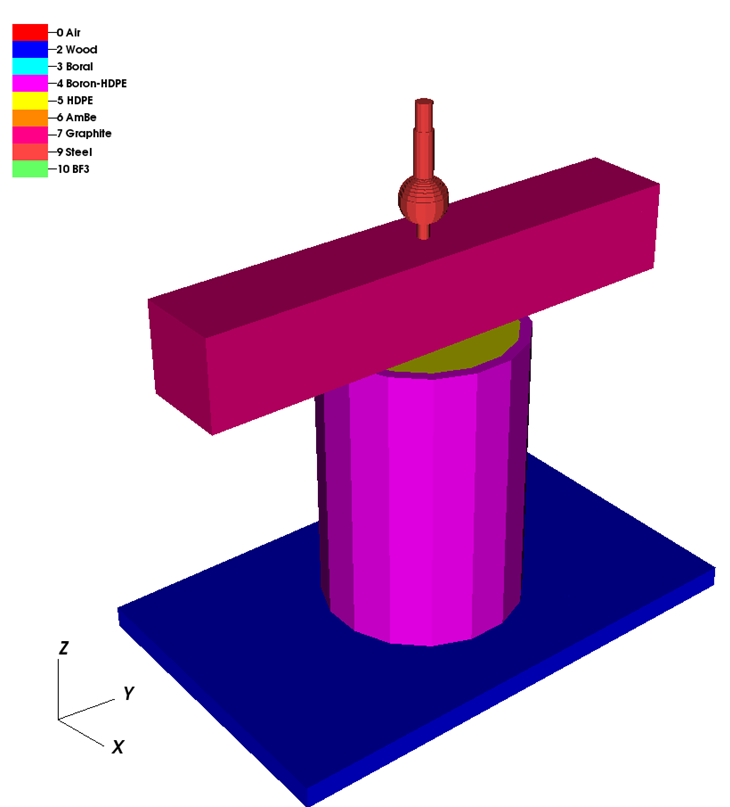
\includegraphics[scale=0.25]{figures/IM1_3D_extrude.png}
\end{frame}

\begin{frame}[t]\frametitle{Extruded Mesh Capability}
\centering
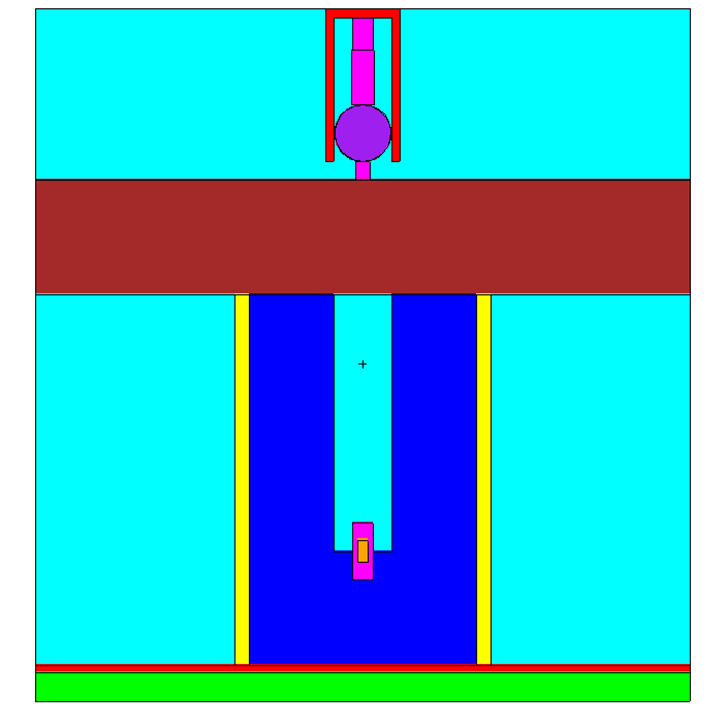
\includegraphics[scale=0.23]{figures/IM1_MCNP}
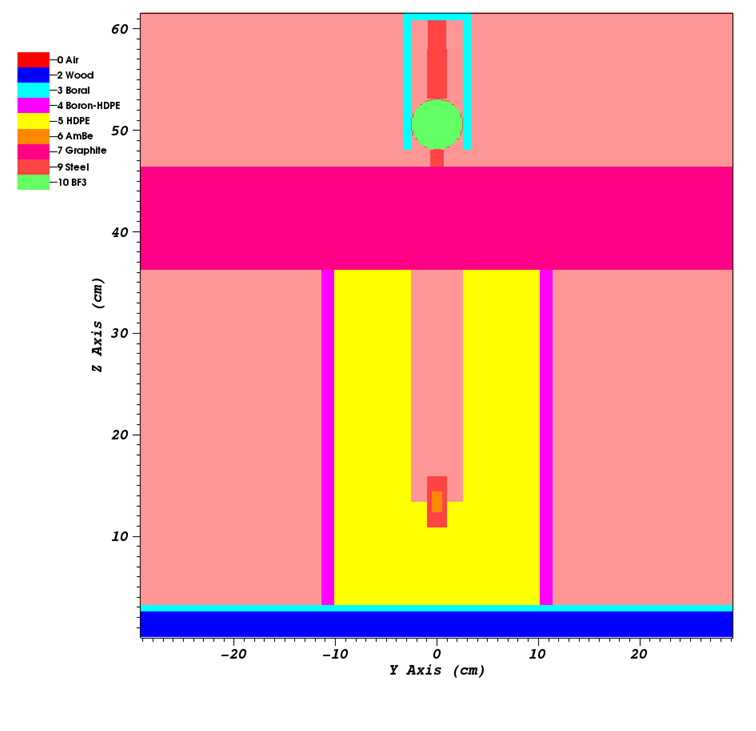
\includegraphics[scale=0.23]{figures/IM1_PDT}
\end{frame}

\begin{frame}[t]\frametitle{MCNP vs. PDT}
\begin{table}[H]
\centering
\small
\caption{The results of MCNP and PDT Compared for IM1-B}
\begin{tabular}{c | c | c}
\hline
\textbf{Code and Setup} & Abs. Rate w/Air ($s^{-1}$) & Abs. Rate w/Graphite $s^{-1}$\\
\hline
MCNP & 70.1 & 12.66 \\
PDT Unstructured & 68.93 & 12.75 \\
\hline

\end{tabular}
\end{table}
\end{frame}



\begin{frame}[t]\frametitle{Conclusions}
\begin{block}{}
\begin{itemize}
\item The effectiveness of the load balancing algorithm depends on the spatial distribution of fine geometric features, the maximum triangle area used, and the number of subsets the domain is decomposed into.
\item Good improvement is seen for all test cases, particularly the first two. 
\item Improvements to the algorithm must be made, as the user will often need to decide on the number of subsets based on how many processors are wanted. 
\end{itemize}
\end{block}
\end{frame}

\begin{frame}[t]\frametitle{Future Work}
\begin{block}{}
\begin{itemize}
\item Three paths for improving the load balancing algorithm have been outlined.
\begin{itemize} 
\item Adaptively splitting the subsets that have large cell counts into smaller subsets, and redistributing subsets amongst processors.
\item Load balancing by column only, then in each column individually load balancing rows. 
\item Taking advantage of nested parallelism to assign more parallel processes at subsets that require more work to be done.
\end{itemize}
\end{itemize}
\end{block}
\end{frame}

\begin{frame}[t]\frametitle{Initial Setup}
\centering
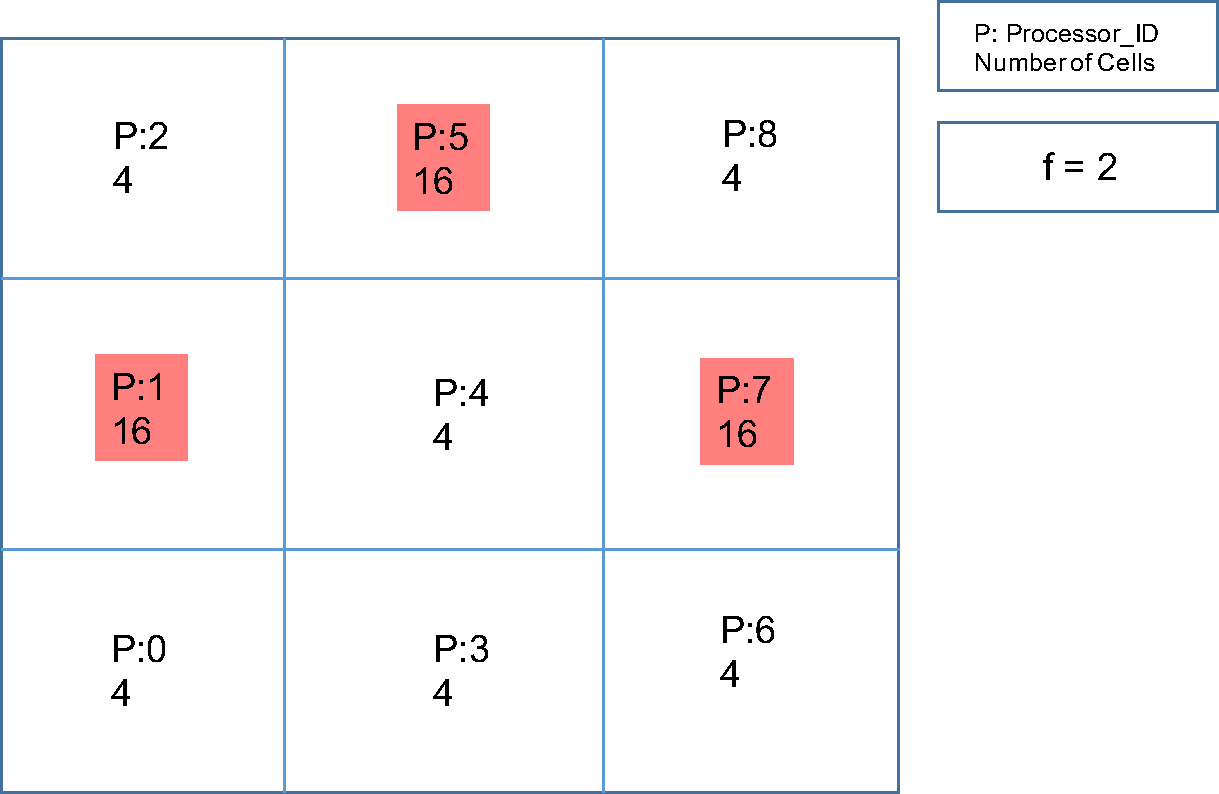
\includegraphics[scale=0.5]{figures/initial_setup.pdf}
\end{frame}

\begin{frame}[t]\frametitle{Adaptively Refine Subsets}
\centering
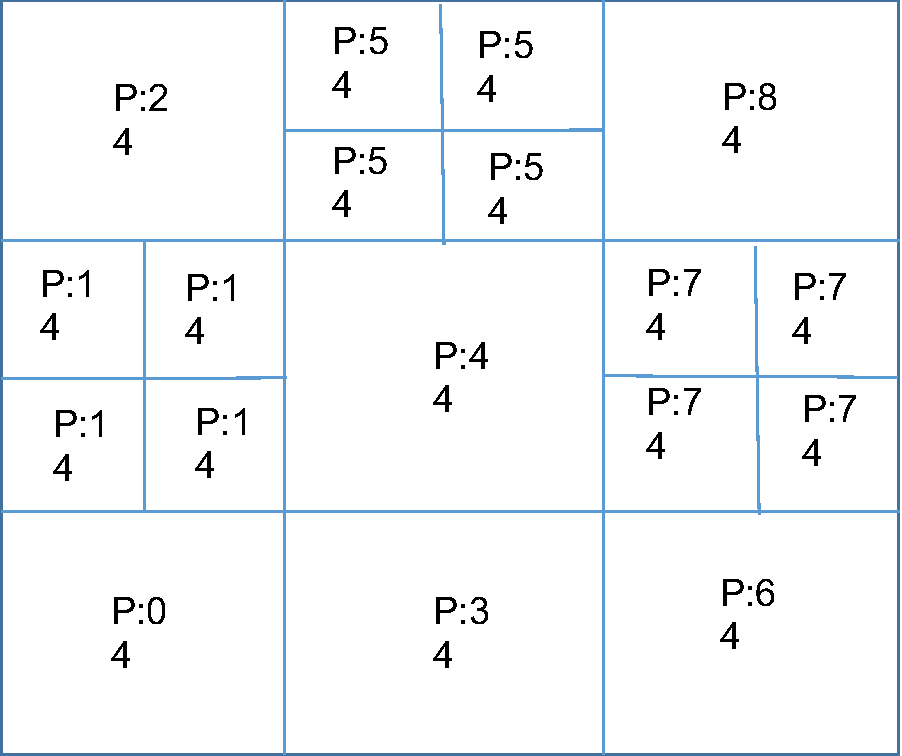
\includegraphics[scale=0.5]{figures/amr.pdf}
\end{frame}

\begin{frame}[t]\frametitle{Subset Redistribution}
\begin{minipage}{0.15\textwidth}
\begin{footnotesize}
$f = 1$
\end{footnotesize}
\end{minipage}
\begin{minipage}{0.8\textwidth}
\centering
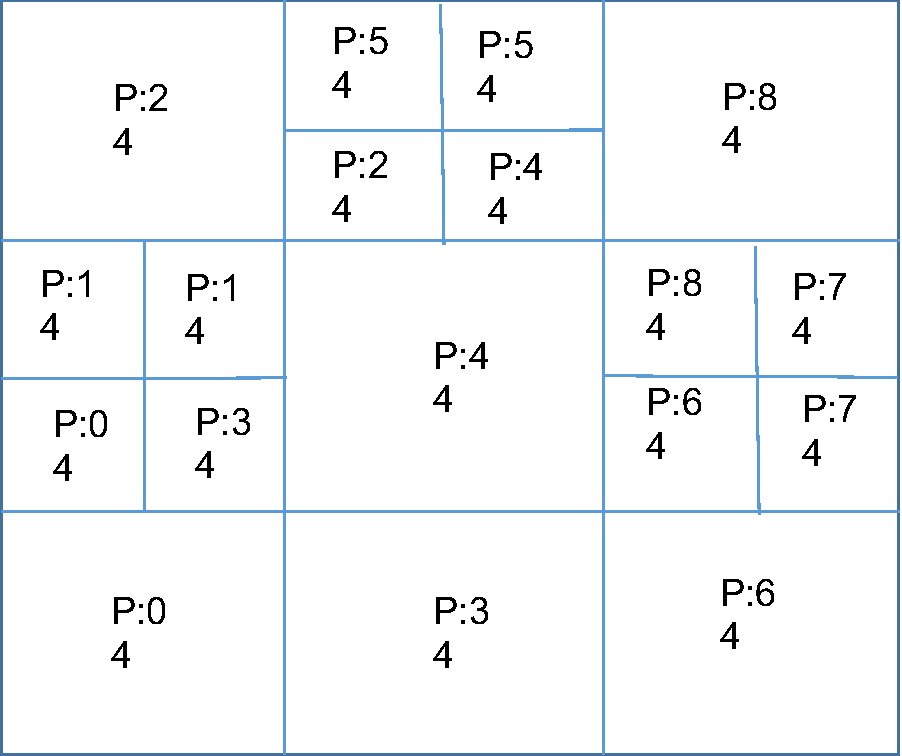
\includegraphics[scale=0.5]{figures/domain_overloading.pdf}
\end{minipage}
\end{frame}

\begin{frame}[t]\frametitle{Load Balancing by Dimension}
\centering
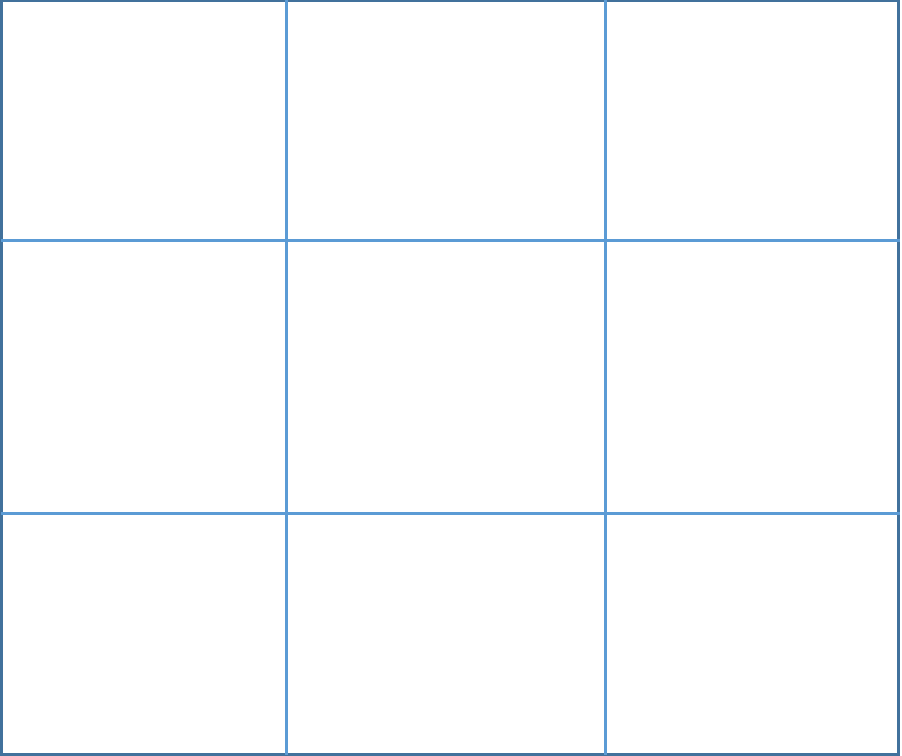
\includegraphics[scale=0.5]{figures/initial_1b.pdf}
\end{frame}

\begin{frame}[t]\frametitle{Load Balance Columns}
\centering
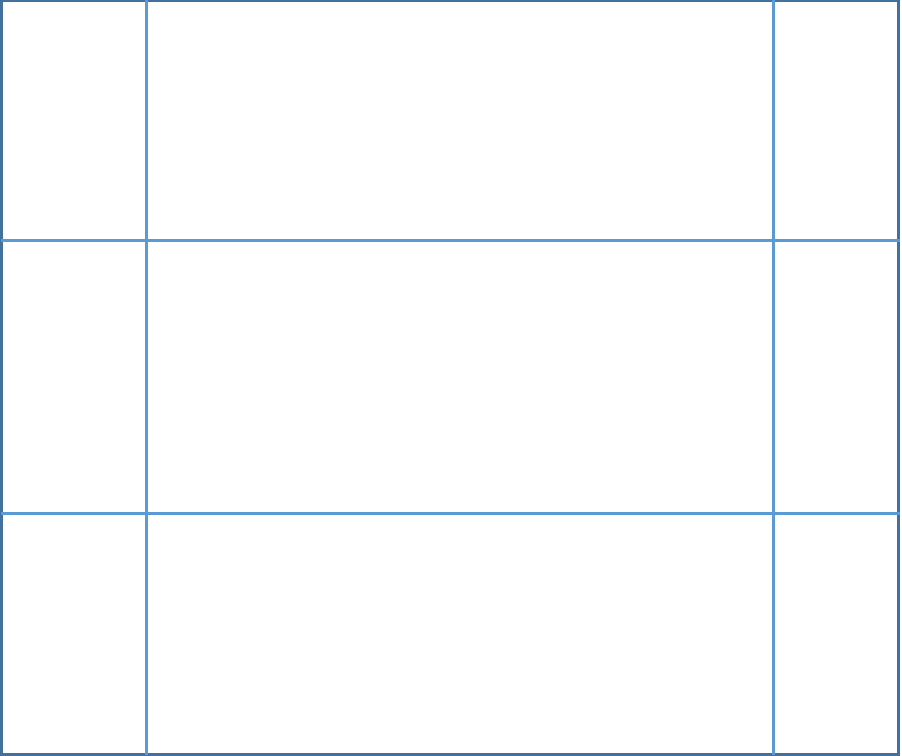
\includegraphics[scale=0.5]{figures/row_moves.pdf}
\end{frame}

\begin{frame}[t]\frametitle{Load Balancing by Dimension}
\centering
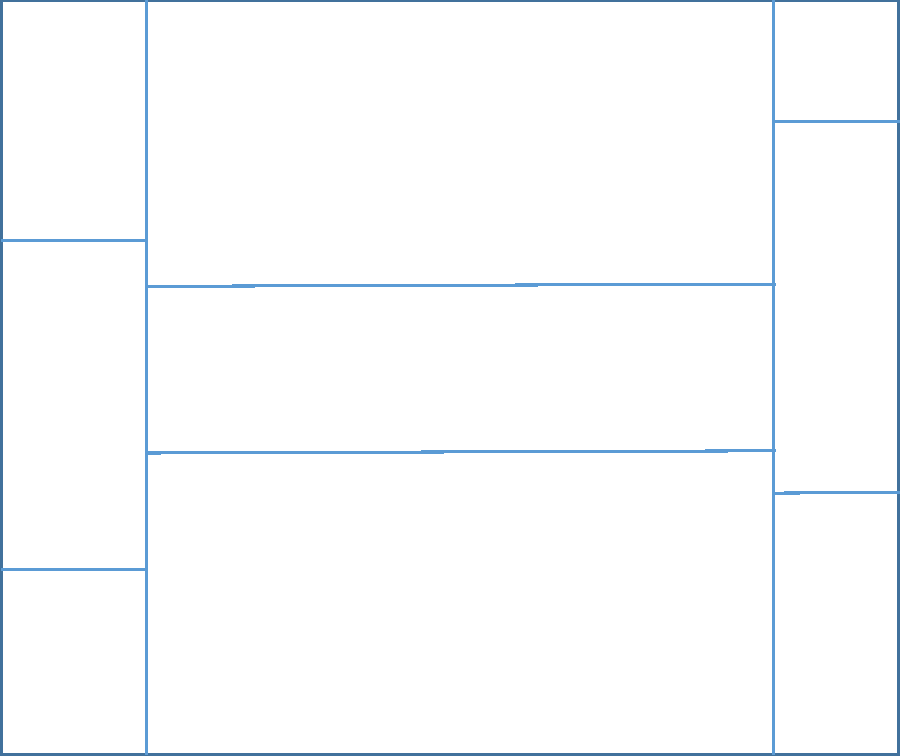
\includegraphics[scale=0.5]{figures/column_moves.pdf}
\end{frame}


\begin{frame}[t]\frametitle{Nested Parallelism}
\centering
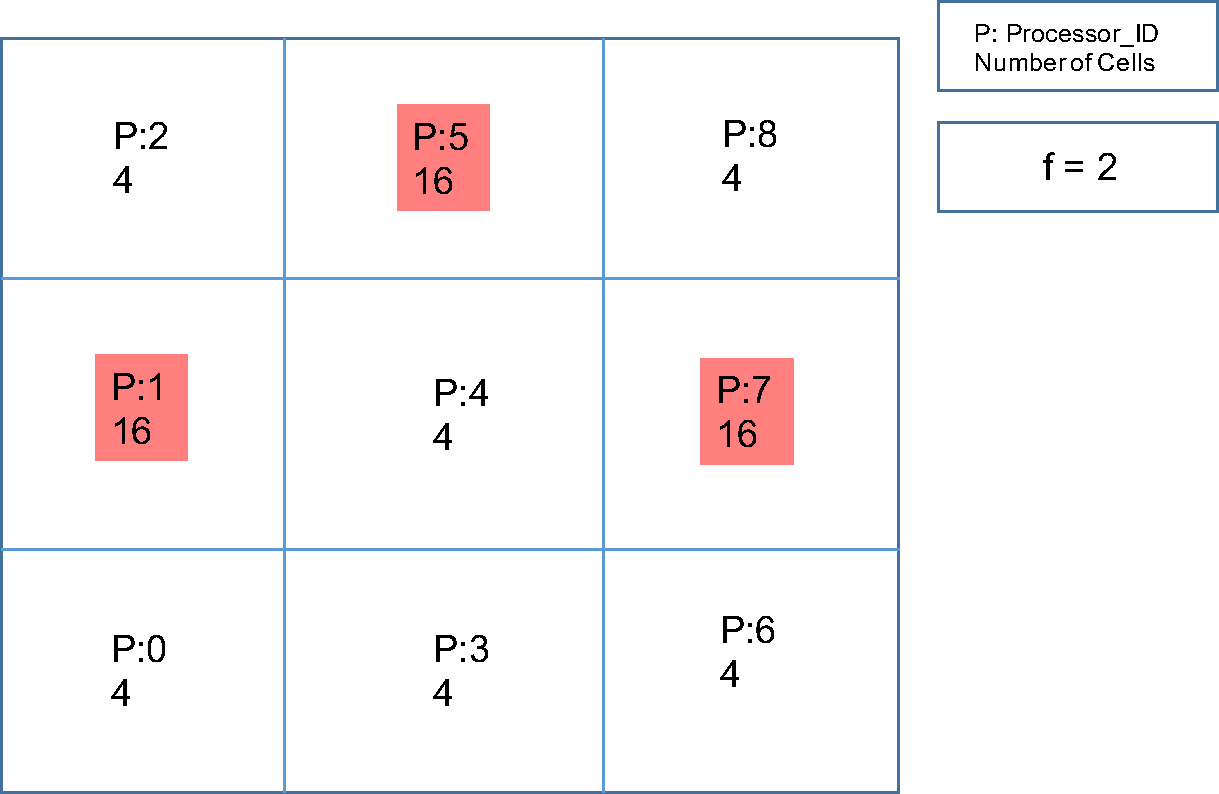
\includegraphics[scale=0.5]{figures/initial_setup.pdf}
\end{frame}

\begin{frame}[t]\frametitle{Acknowledgements}
\begin{block}{}
A special thank you to the following individuals for their help and support:
\begin{itemize}
\item Drs. Ragusa, Morel, Adams, and Popov
\item Michael Adams, Daryl Hawkins, and Dr. Timmie Smith
\item Dr. Andrew Till
\item The CERT team and fellow grad students
\item PSAAP-II 
\end{itemize}
\end{block}
\end{frame}

\backupbegin
\appendix
\section{Backup Slides}
\begin{frame}[t]\frametitle{Backup Slides}

\end{frame}

\begin{frame}[t]\frametitle{Solution Verification}
\begin{block}{}
\begin{itemize}
\item Two benchmark problems were set up to verify that the scalar flux was being computed correctly on unstructured meshes in PDT.
\item Both problems utilized a 1 cm$\times$1 cm square domain, with opposing reflecting boundaries on the y boundaries, an incident isotropic angular flux on the left boundary, and a vacuum boundary on the right.
\end{itemize}
\end{block}
\begin{block}{}
The error presented when comparing numerical to analytical solutions is defined as follows:
\begin{align*}
\epsilon = \frac{\norm{\text{Analytical} - \text{ Numerical}}_{l2}}{\norm{\text{Analytical}}_{l2}},
\end{align*}
\end{block}
\end{frame}

\begin{frame}[t]\frametitle{Pure Absorber}
\begin{block}{}
The analytical scalar flux solution of the 1D Pure Absorber is:
\begin{align*}
\phi(x) &= \int_{0}^{1}\psi(x,\mu>0) d\mu \notag \\
&= \int_{0}^{1}\psi_{inc}\exp(-\frac{\Sigma_a}{\mu} x) d\mu = \psi_{inc} E_{2}(\Sigma_a x),
\end{align*}
\end{block}
\begin{block}{}
The pure absorber was run with $\psi_{inc} = 3.5 \frac{\text{n}}{\text{cm}^2\text{-s-ster}}$ and $\Sigma_a = 5 \text{ cm}^{-1}$.
\end{block}
\end{frame}

\begin{frame}[t]\frametitle{PDT Results vs. Analytical for the Pure Absorber}
\centering
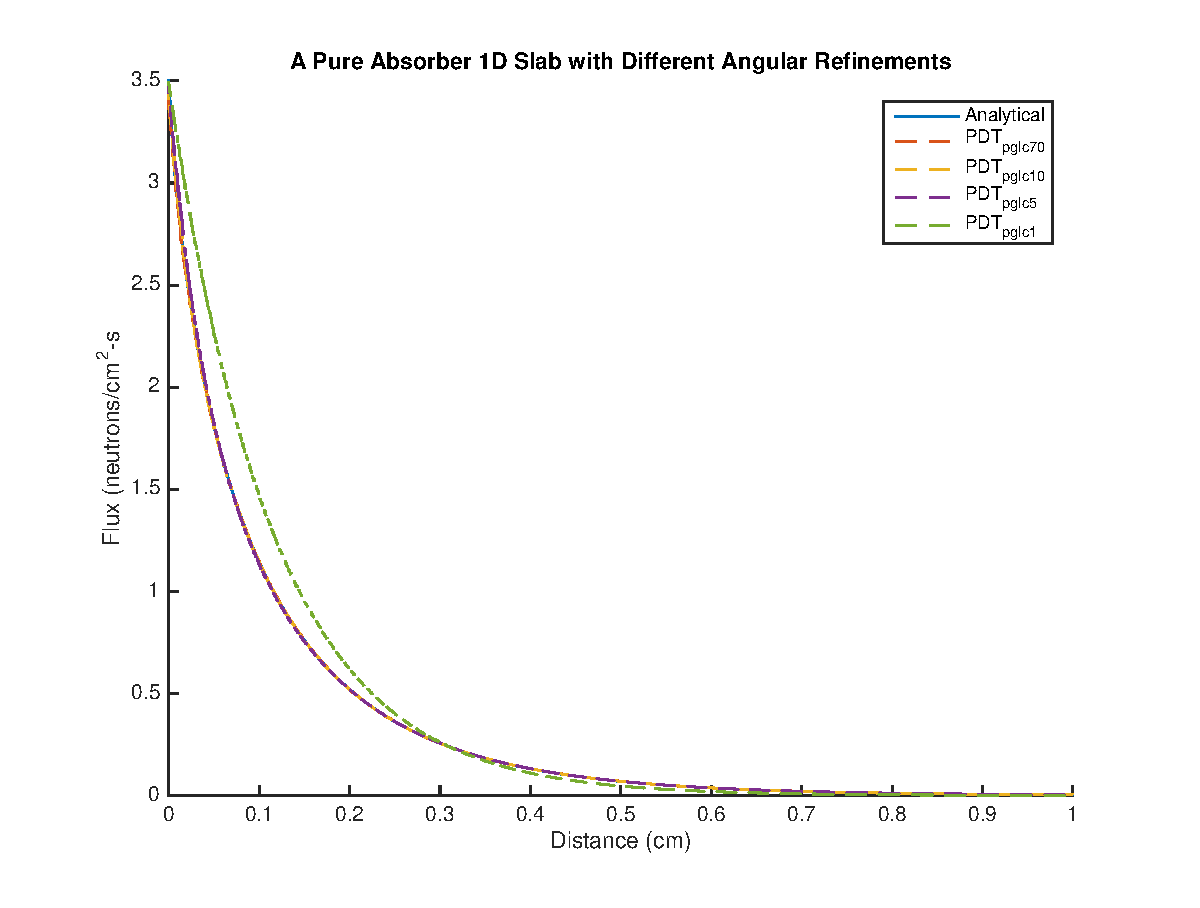
\includegraphics[scale = 0.5]{figures/PureAbsorberAllAngles.eps}
\end{frame}

\begin{frame}[t]\frametitle{Analysis with 70 Positive Polar Angles}
\begin{minipage}{0.15\textwidth}
\begin{footnotesize}
$\epsilon = 0.012$
\end{footnotesize}
\end{minipage}
\begin{minipage}{0.8\textwidth}
\centering
\includegraphics[scale = 0.5]{figures/PureAbsorberBestangle.eps}
\end{minipage}
\end{frame}

\begin{frame}[t]\frametitle{Pure Scatterer}
\begin{block}{}
The transport solution for a pure scatterer reaches the diffusion limit, and the solution is:
\begin{align*}
\phi(x) = \frac{4j_{inc}}{1+4D}(-x + x_{\text{max}} + 2D).
\end{align*}
\end{block}
\begin{block}{}
This problem was run with $\Sigma_t = 100 \text{ cm}^{-1}$ and $j_{inc} = \frac{7}{4} \frac{\text{n}}{\text{cm}^2\text{-s}}$. 
\end{block}
\end{frame}

\begin{frame}[t]\frametitle{PDT Results vs. Analytical for the Pure Scatterer}
\begin{minipage}{0.2\textwidth}
\begin{footnotesize}
$\epsilon$=4.25E-04
\end{footnotesize}
\end{minipage}
\begin{minipage}{0.75\textwidth}
\centering
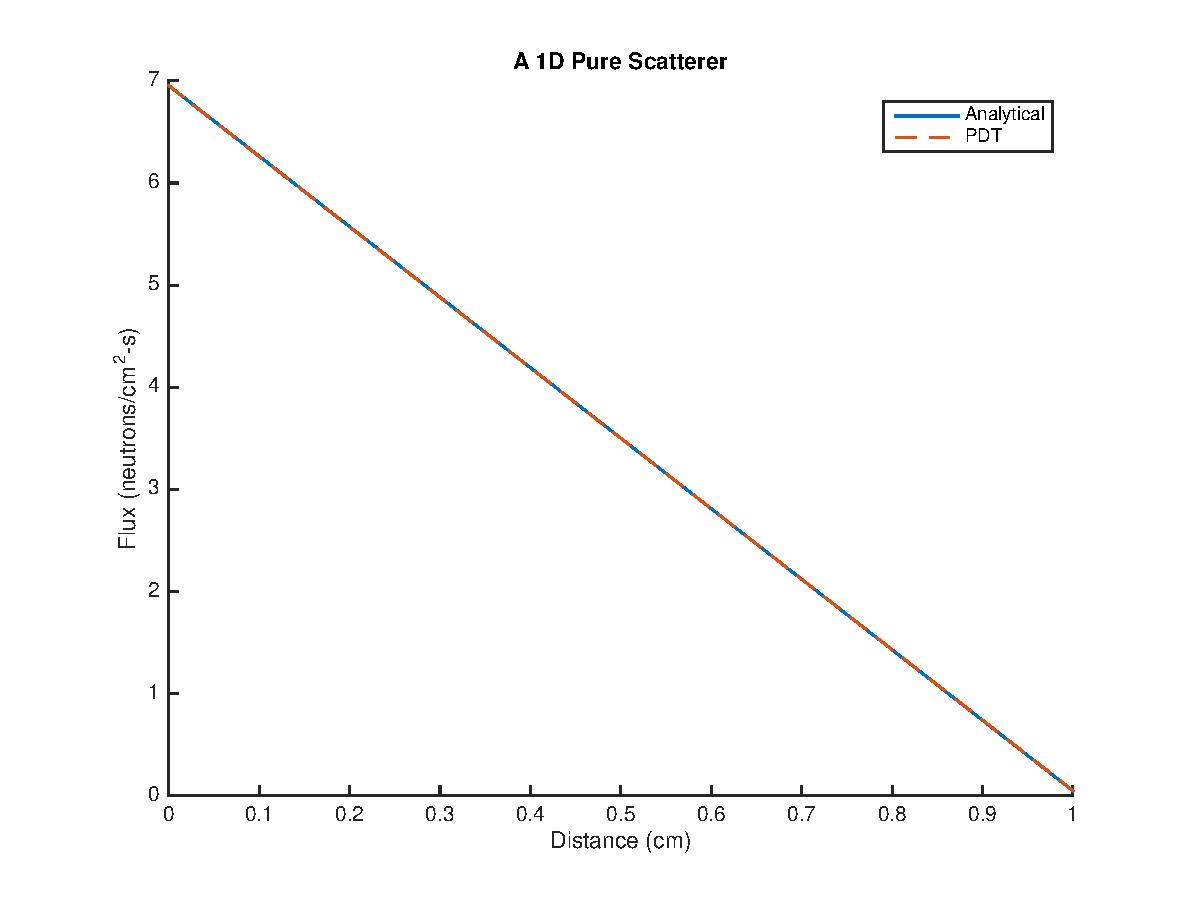
\includegraphics[scale = 0.5]{figures/PureScatterer.eps}
\end{minipage}

\end{frame}


\backupend

%\begin{frame}[allowframebreaks]{Bibliography}
%\bibliographystyle{alpha}
%\bibliography{science}
% \nocite{*}
%\end{frame}



%\section{\ }
%\begin{frame}[t]\frametitle{Sources}
%	\nocite{Dubcova20111182}
%	\nocite{CHAUVET}
%	\bibliographystyle{ieeetr}
%	\bibliography{science.bib}
%	
%	
%\end{frame}
%



\end{document}